\author{Bianca Ploch}
\title{Mobile Display of Knitting Patterns}

\newcommand{\thesistitle}{Mobile Display of Knitting Patterns}
\newcommand{\studiengang}{International Media and Computing}
\newcommand{\thesisauthor}{Bianca Ploch}
\newcommand{\fachbereich}{Wirtschaftswissenschaften II}
\newcommand{\matrikelnr}{540609}
\newcommand{\firstsupervisor}{Prof. Dr. Debora Weber-Wulff}
\newcommand{\thesisyear}{2016}

\newcommand{\refchapter}[1]{\textbf{\hyperref[#1]{\ref*{#1}: \nameref{#1}}}}
\newcommand{\reflisting}[1]{\textit{\hyperref[#1]{Listing ~\ref*{#1}}}}
\newcommand{\refweb}[2]{\textit{\textbf{\href{#1}{#2}}}}
\newcommand{\reffigure}[1]{\textbf{\hyperref[#1]{Figure \ref*{#1}}}}
\newcommand{\code}[1]{\texttt{#1}}
\newcommand{\sectionheading}[1]{\noindent{\textbf{#1}}}
\documentclass[
  a4paper,
  oneside,
  titlepage,
  11pt
]{memoir}

\PassOptionsToPackage{hyphens}{url}\usepackage[breaklinks=true]{hyperref} % for all the refs (chapter, website)
\usepackage{listings}   % for code
\usepackage{multicol}
\usepackage{caption}    % all the captions
\usepackage[list=true]{subcaption}
\usepackage{color}      % for proper color handling
\usepackage{todonotes}  % for notes
\usepackage[toc,acronym]{glossaries} % for the glossary
\usepackage{graphicx}   % for advanced image handling
\usepackage{fixltx2e}   % for subscript
\usepackage{amssymb,amsmath} % for math equations
\usepackage{lscape}     % for landscape pages
\usepackage{breakcites} % breaks overfloating cites
\usepackage{wrapfig}
\usepackage{soul}

\usepackage{float}
\usepackage[utf8]{inputenc}
\usepackage{url}
\usepackage{csquotes}
\usepackage{geometry}
\usepackage{ltablex} % for table that spans more than one page
\PassOptionsToPackage{hyphens}{url}
\usepackage{hyperref} %breaking url at line end
\usepackage{breakurl}

\usepackage{tocloft} 
\usepackage[
	backend=biber,
	style=authortitle,
	citestyle=authoryear
]{biblatex}
 
\addbibresource{biblio.bib} %Imports bibliography file

\setsecnumdepth{subsubsection}
\settocdepth{subsubsection}
\setcounter{lofdepth}{2}

\usepackage{enumitem}
\definecolor{javared}{rgb}{0.6,0,0} % for strings
\definecolor{javagreen}{rgb}{0.25,0.5,0.35} % comments
\definecolor{javapurple}{rgb}{0.5,0,0.35} % keywords
\definecolor{javadocblue}{rgb}{0.25,0.35,0.75} % javadoc
\definecolor{darkblue}{rgb}{0.12,0,0.58}
\definecolor{xmlgreen}{rgb}{0,0.6,0}
\definecolor{xmlblue}{rgb}{0.25,0,1}
\definecolor{androidpurple}{rgb}{0.53,0,0.55}



% settings
\lstset{language=Java,
  basicstyle=\footnotesize\ttfamily,
  % basicstyle=\ttfamily,
  keywordstyle=\color{javapurple}\bfseries,
  stringstyle=\color{javared},
  commentstyle=\color{javagreen},
  morecomment=[s][\color{javadocblue}]{/**}{*/},
  frame=lines,
  numbers=left,
  breaklines=true,
  numberstyle=\tiny\color{black},
  % numberstyle=\footnotesize,
  stepnumber=1,
  captionpos=b,
  numbersep=10pt,
  tabsize=2,
  % margin
  xleftmargin=19pt,
  aboveskip=15pt,
  % belowskip=15pt,
  showspaces=false,
  showstringspaces=false
}

\lstdefinelanguage{XML}
{
  basicstyle=\footnotesize\ttfamily\color{darkblue}\bfseries,
  morestring=[b]",
  frame=lines,
  stringstyle=\color{xmlgreen},
  identifierstyle=\color{darkblue},
  keywordstyle=\color{xmlblue},
  moredelim=[s][\color{black}]{>}{<},
 % moredelim=[s][\color{androidpurple}]{\ }{:},
  morekeywords={xmlns,version,type,name,format,android}% list your attributes here
  }
  
  \lstdefinelanguage{struct}
{
  basicstyle=\tiny\ttfamily
  }
  
  \lstdefinelanguage{XML_appendix}
{
  basicstyle=\tiny\ttfamily\color{darkblue}\bfseries,
  morestring=[b]",
  frame=lines,
  stringstyle=\color{xmlgreen},
  identifierstyle=\color{darkblue},
  keywordstyle=\color{xmlblue},
  moredelim=[s][\color{black}]{>}{<},
 % moredelim=[s][\color{androidpurple}]{\ }{:},
  morekeywords={xmlns,version,type,name,format,android}% list your attributes here
  }
  

\linespread{1.3}        % one and a half

\makeglossaries
\glsaddall
\newacronym{RS}{RS}{right side}
\newacronym{WS}{WS}{wrong side}
\newacronym{json}{JSON}{JavaScript Object Notation}
\newacronym{GUI}{GUI}{Graphical User Interface}
\newacronym{IDE}{IDE}{Integrated Development Environment}
\newacronym{SDK}{SDK}{Software Development Kit}
\newacronym{API}{API}{Application Programming Interface}
\newacronym{UI}{UI}{User Interface}
\makeglossaries
\begin{document}

%!TEX root = ../thesis.tex

\thispagestyle{empty}

%\begin{titlepage}

\begin{center}

\vspace*{2cm}
\Large
\textsc{\thesistitle}\\

\vspace{3cm}

%\LARGE
\textsc{Bachelor's Thesis\\[0.5\baselineskip]
%\\[0.5\baselineskip]
\thesisauthor\\
\matrikelnr}\\


\vspace{2.5cm}
\textsc{16 August 2016}\\

\vspace{1cm}
\textsc{Supervisor:\\
\firstsupervisor}\\

\vspace{0.5cm}
\textsc{HTW Berlin\\
International Media and Computing (Bachelor)}

\end{center}

%\end{titlepage}
% Keine Seitenzahl für diese Seite
\addtocounter{page}{-1}

% \noindent \textbf{Acknowledgements}
\thispagestyle{empty}
\vspace*{1cm}

\noindent
I would like to express my sincere gratitude to my supervisor, \firstsupervisor \, for the continuous support and guidance given to me during this thesis.\\

\medskip\noindent
Besides my supervisor, I would also like to thank my proof-readers, Tu Le-Than, Tormod Gjeitnes Hellen, and Joakim Uddholm, for their hard work.\\

\medskip\noindent
Furthermore, I would like to thank Nadine Kost, Thilo Ilg, and Angela Thomas for their time and participation in the user interviews and testing.\\

\medskip\noindent
Last but not least, I would like to thank my family and friends for cheering me on and supporting me at all times.

\addtocounter{page}{-1}

\pagenumbering{roman}
\setlength{\cftparskip}{-0.5pt}
\tableofcontents

\pagenumbering{arabic}

\chapter{Introduction}
Since the beginning of the 2000s, knitting has encountered a steady rise in popularity, claims an article by \cite{lewis_rise_of_knitting}. This, she says, might be due to the rise of the internet and social media, and the increasingly important role they play in the daily life. The older knitting generation is adapting to new technology and switching over, Nielsen explains, bringing knitting as a craft and hobby closer to the younger generations (\cite{lewis_rise_of_knitting}). Online communities like Ravelry\footnote{\url{http://www.ravelry.com/}} and Youtube\footnote{\url{https://www.youtube.com/}} teach the knitting enthusiasts knittings techniques and patterns of all kinds --- never has knitting knowledge been more accessible.

Considering this, it is all the more surprising that there are only few apps related to knitting to be found on the Play Store, Google's digital distribution service for Android apps. Only one app supports the creation of a knitting pattern chart. Mobile devices have the potential to be a great help to knitters. An app could help knitters keep track of the projects they are currently knitting, look up instructions, and store knitting patterns. The latter especially aids the mobile knitter --- no longer is it necessary to carry sheets of paper with pattern charts or even books, as seen in \reffigure{fig:knitting_book}, around.

\begin{figure}[H]
	\centering
    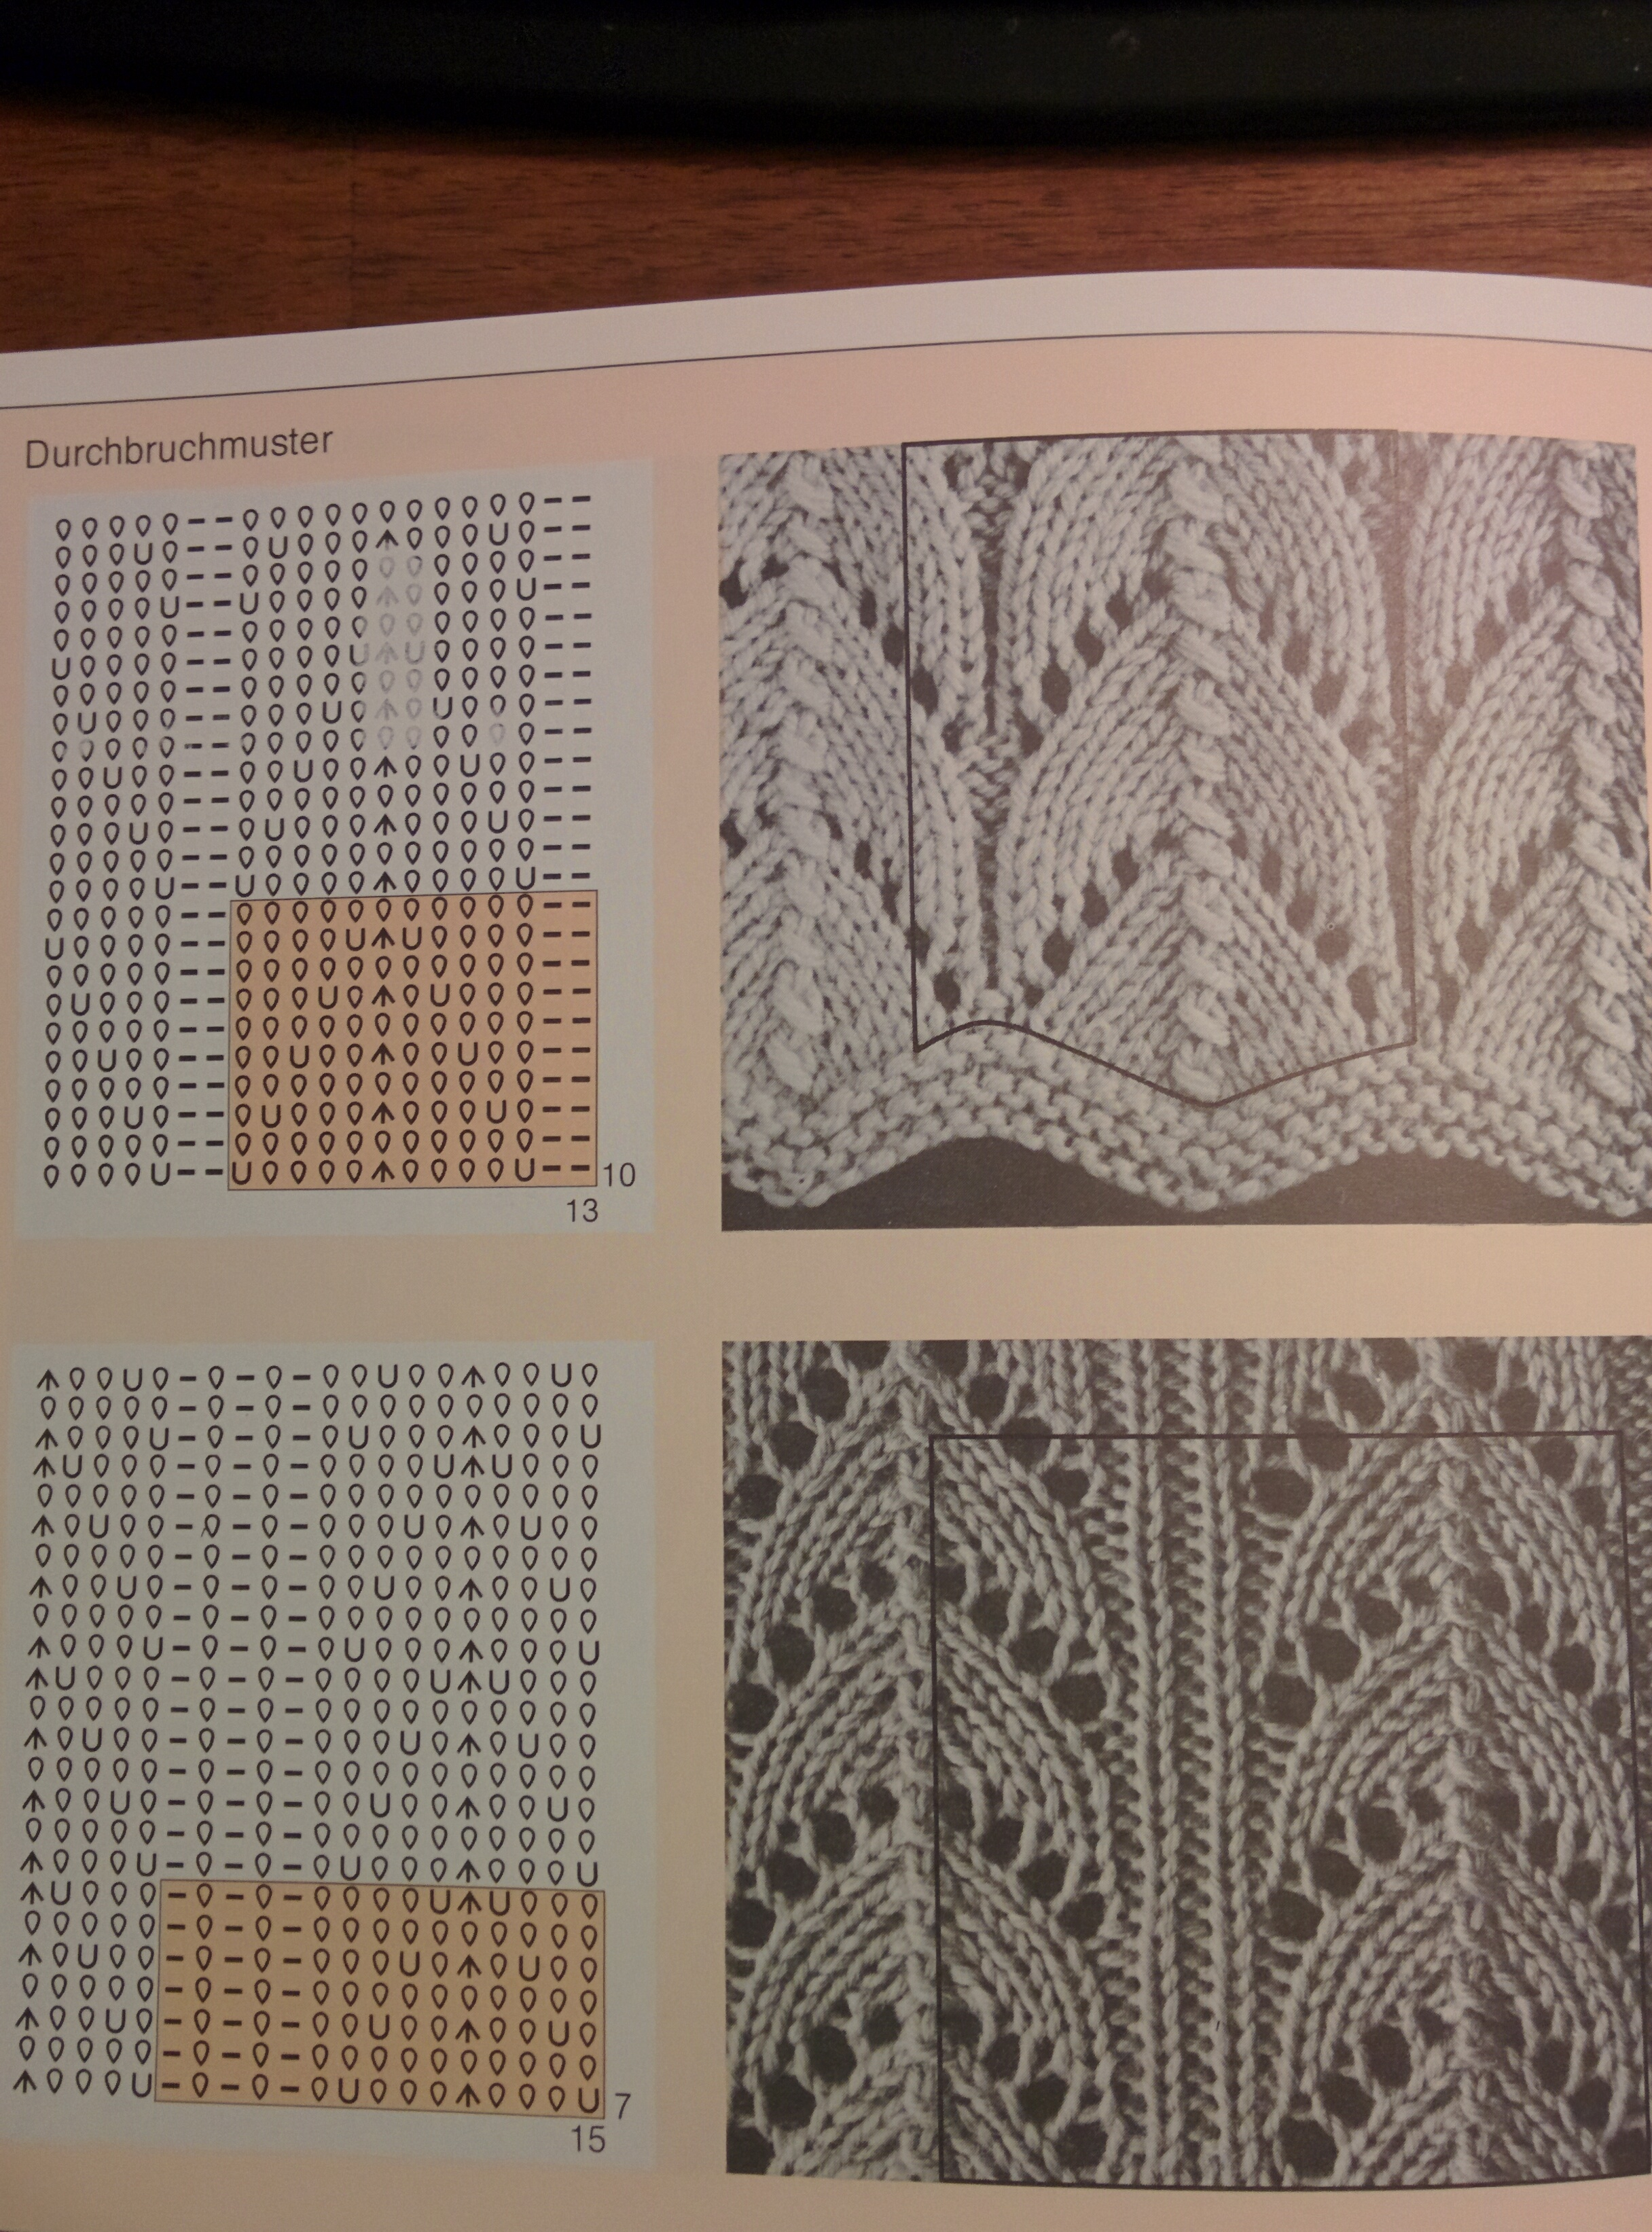
\includegraphics[width=.45\textwidth]{images/knitting_pattern_chart_book.jpg}
   \caption[{Knitting patterns and their corresponding pattern charts \protect\newline{\small from \protect\cite[p142]{Natter1983}}}]{Knitting patterns and their corresponding pattern charts from \protect\cite[p142]{Natter1983}}
   \label{fig:knitting_book}
\end{figure}

The difficulty with displaying such a chart on a mobile device is due to the size of the device's screen. This screen is a far smaller medium than a sheet of paper, on which pattern charts are normally printed. 

Pattern charts, excluding the smaller charts, are therefore too big to be viewed easily inside an app. The goal for this thesis is to research how a knitting pattern chart can be input and displayed on mobile devices running the Android operating system and develop a working prototype showcasing the results of that research. The prototype will be evaluated through testing by users representative of the prototype's target group. This testing will, if time permits, executed iteratively throughout developement to ensure a useful \gls{UI} design. The term useful in this context is taken from the article \textit{Usability 101: Introduction to Usability} by \cite{nielsen2014} --- he uses the term to summarize the usability and utility of a design. Nielsen furthermore defines utililty and usability as indicators of ``[...] whether [a design] provides the features you need'' and ``how easy [and] pleasant these features are to use'' (\cite{nielsen2014}).

\chapter{Background}
\section{Definition of Knitting Pattern and Knitting Pattern Chart}

A knitting pattern specifies a set of instructions outlining the steps necessary to create a knitted textile or fabric. For knitting a fabric the knitter uses two or more knitting needles and a long, continuous strand of yarn which he uses to form intersecting loops with, which in turn creates a textile or fabric. ``Knitting is a conversion system in which yarn loops are interwoven to form a fabric'' ~\cite[p17]{Raz1993}. The type of loops the knitter uses as well as the kind of yarn determine the attributes of the knitted piece: elasticity, form and texture. A knitted fabric can be stretched in both horizontal and vertical directions, as well as the directions in-between. This makes it stand apart from woven fabric, which is created by layering two threads in an interlaced manner; the resulting cloth is very limited in its ability to stretch and be formed, excluding, of course, the usage of stretching threads. 
Knitting patterns can come in form of written instructions, usually with abbreviations used for the stitch terms, e.g. k2tog for the ``knit two together'' stitch, or in form of a pattern chart which consists of a grid filled with symbols. Both, written patterns and pattern charts, are generally split into rows, where each row has a definite number of stitches. Each cell in such a grid signifies a stitch in the pattern and the symbol displayed in a cell corresponds with the stitch that needs to be made in that place in the pattern. In what order the rows have to be knitted depends on the chart type; some charts display only the uneven numbered rows, which belong to the \gls{RS} of the knitted fabric, and expect the knitter to knit the return row on the \gls{WS} inverse to the \gls{RS}, i.e. knits would be knitted as purls and purls as knits. Other charts show all rows, the uneven numbered for the \gls{RS} and the even numbered ones for the WS.

So far there doesn't exist an international standard for the symbols used in knitting charts or the abbreviations in written instructions. Symbols used by the industry usually vary depending on the region ~\cite[p57]{Raz1993}. and it is the norm that a knitting pattern includes a glossary for the symbols and abbreviations used in the pattern. Singular exception to this is Japan, where there exists a Japanese Industrial Standard on knitting symbols used in the industry and for the hobby hand knitters: JIS L 0201-1995~\cite{JKCA1995}. This leads to the fact that Japanese knitting pattern charts are published without an index of the symbols used.

Other regional industry standards that Raz mentions in his book are the German Standard and the needle notation system, ``the most explicit and accurate of all  notation systems'' ~\cite[p58]{Raz1993}., which is solely used for industrial knitting and shows the positions of the needles of the knitting machine for each stitch.

\section{Comparison of existing Android solutions}

\subsection{Android apps}
When searching for the term ``knitting'' in the Google Play Store, Android’s official source for Google-approved applications, few results will pop up. Next to a surprising amount of games about knitting, there are apps for knitting counters, knitting patterns and knitting instructions for those who wish to begin knitting. The following sections will look at the top five apps for creating and managing knitting projects with row counters and pattern display, as well as knitting chart creation.

\addcontentsline{toc}{subsubsection}{knit tink | Row Counter by Jennifer K. Warren}
\subsubsection*{knit tink | Row Counter by Jennifer K. Warren}
Out of all most popular knitting apps, knit tink features the most modern and clean design. The app can be used for free or bought as an ad-free pro version. Features include the creation, editing, viewing, and deletion of projects, the setup of one row, and one repeat counter per project, as well as the unlinking of the row counter from the repeat counter. The free version of the app restricts the number of projects to three. The developer announced an on-screen display of a knitting chart in PDF format as an upcoming feature.

\begin{figure}[H]
  \centering
    \begin{subfigure}[b]{0.33\textwidth}
      \centering
        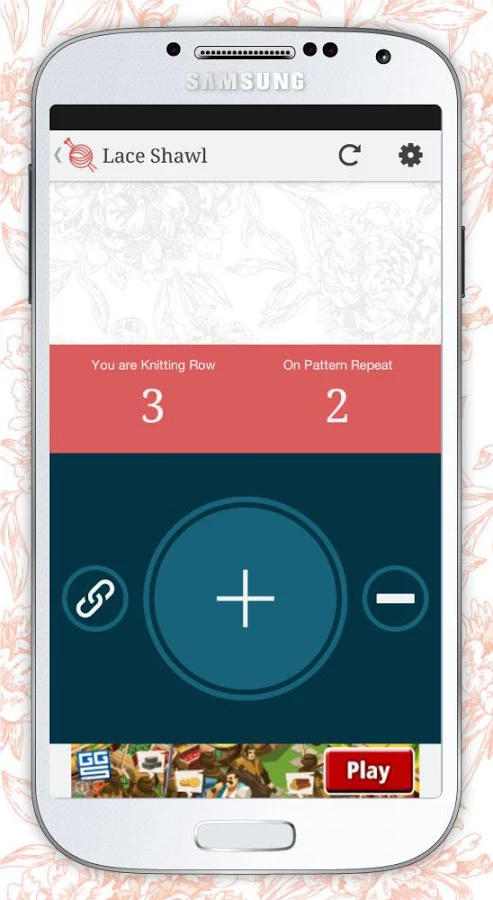
\includegraphics[width=0.95\linewidth]{images/image10.png}
        \caption[Row Counter \protect{\small at: \url{https://lh6.ggpht.com/-9DvA3pUKqPQwDwi8P_mZXOEhyKz9pE4Dks2QuEKxEGJePvXfY4hUkLO0i-zud38c5Y=h900-rw} (last accessed: 2016-04-04)}]{Row Counter}
      \label{fig:knit_tink_row_counter}
    \end{subfigure}
    \begin{subfigure}[b]{0.33\textwidth}
      \centering
        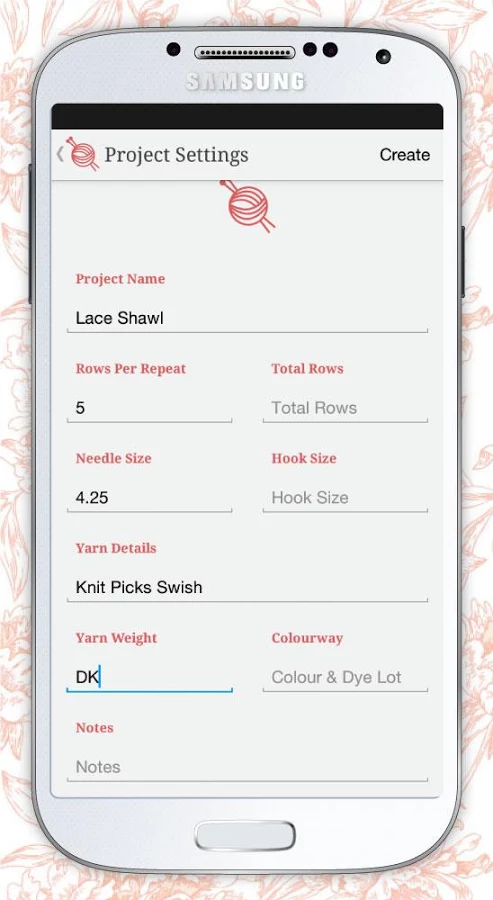
\includegraphics[width=0.95\linewidth]{images/image11.png}
        \caption[Project setup \protect{\small at: \url{https://lh5.ggpht.com/FfgMOtcw2WerHBjS1eqm8NsjuxnTcfPHvxenf-3hfC1NKsIGHp_SPhcQy07Zpru8AQ=h900-rw} (last accessed: 2016-04-04)}]{Project setup}
      \label{fig:knit_tink_project_setup}
    \end{subfigure}
  \caption[Screenshots of the app knit tink \protect{\small at: \url{https://play.google.com/store/apps/details?id=com.warrencollective.knittink} (last accessed: 2016-08-08)}]{Screenshots of the app knit tink}
\end{figure}

\addcontentsline{toc}{subsubsection}{Knitting Counter by mkacki}
\subsubsection*{Knitting Counter by mkacki}
Knitting Counter offers the same features a the knit tink app, the only differences being the layout of the user interface and the option to keep the phone from going into sleep mode, i.e., turning the phone screen off.

\begin{figure}[H]
\centering
\begin{minipage}{.5\textwidth}
  \centering
  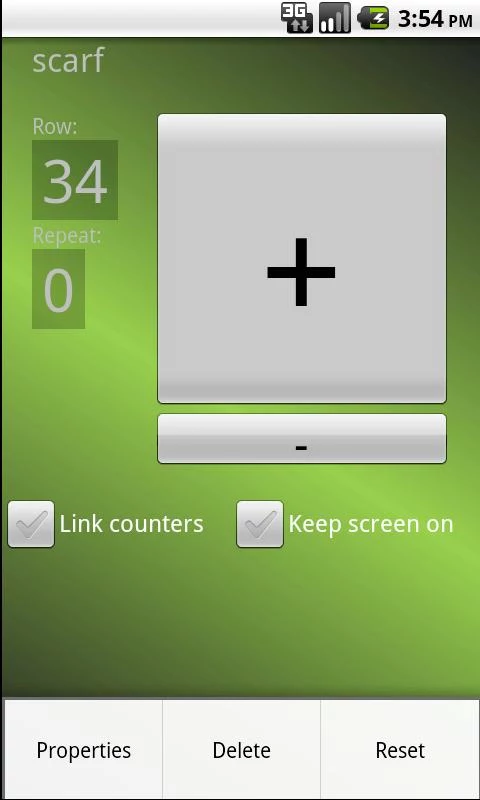
\includegraphics[width=2in]{images/image12.png}
  \caption[Counter of Knitting Counter \protect{\small at: \url{https://lh4.ggpht.com/M05RYCkE7md51ckjB9Bf_CQjz-L6fSS3aWFnQ8UAoURXjO4BuHZiWeHtImzAhhpvekE=h900-rw} (last accessed: 2016-04-04)}]{Counter of Knitting Counter}
  \label{fig_knittingcounter1}
\end{minipage}%
\begin{minipage}{.5\textwidth}
  \centering
  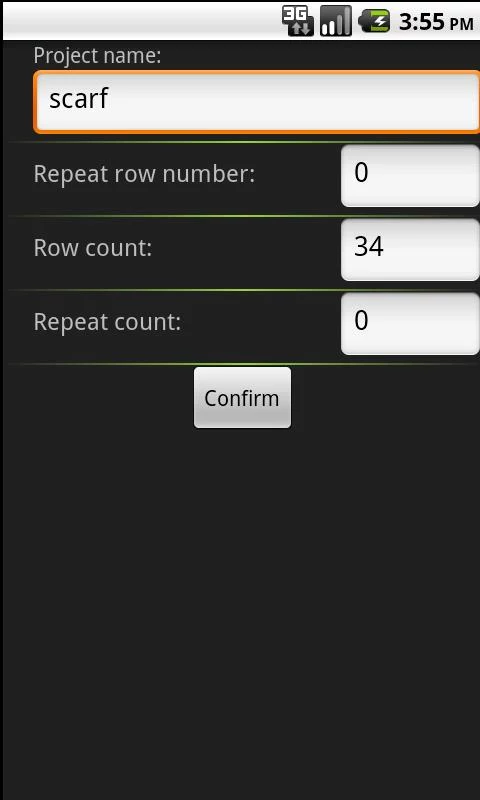
\includegraphics[width=2in]{images/image06.png}
  \caption[Counter set up screen of Knitting Counter \protect{\small at: \url{https://lh3.ggpht.com/AuzeRh7n_r4yLpk9puanH0pBDhcxj6AwC8h5qCaMN3TsRMRu7rML9awuPZTf49M_ejo=h900-rw} (last accessed: 2016-04-04)}] {Counter set up screen of Knitting Counter}
  \label{fig_knittingcounter2}
\end{minipage}
\end{figure}

\subsubsection{Knitting and Crochet Buddy by Colorwork Apps}
The Knitting and Crochet Buddy contains a plethora of features related to knitting and crocheting. As is the standard with the previous apps, it offers the possibility to manage different knitting and crocheting projects, with each a row and a repeat counter per project. Users can also enter written instructions or add a picture of the pattern chart to be displayed on the counter screen.

Additional features include, but are not limited to: yarn and crochet charts, an abbreviation chart, size charts for knitting needles and crocheting hooks, a project timer, a ruler function, and a flashlight.

\begin{figure}[H]
\centering
\begin{minipage}{.5\textwidth}
  \centering
  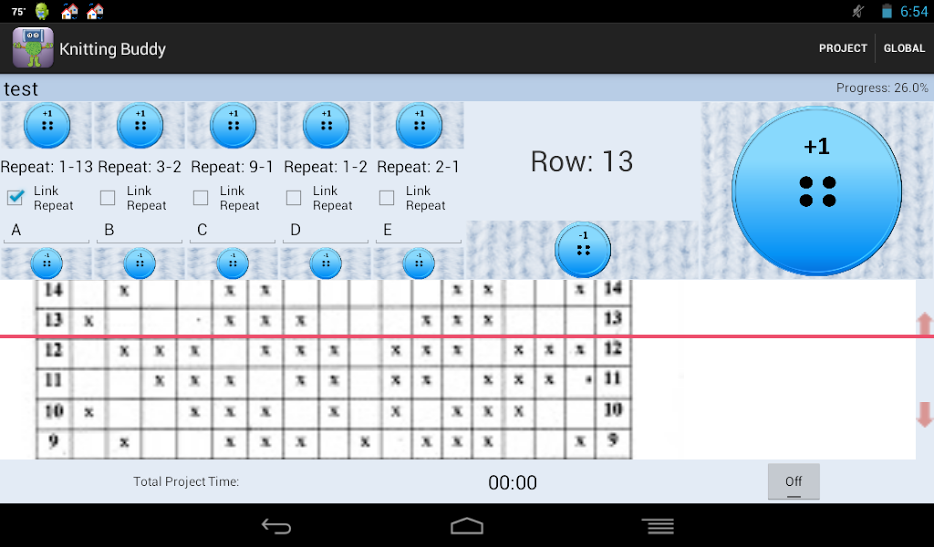
\includegraphics[width=2in]{images/image04.png}
  \caption[Counter of Knitting Buddy with written instructions \protect{\small at: \url{https://lh3.ggpht.com/EPs72ilPpGCF_fMckHsVb2LeYVx-p6eNjcqg69eOwlsS2h0neneeMEpH29CYH3rEM_c_=h900-rw} (last accessed: 2016-04-04)}]{Counter of Knitting Buddy with written instructions}
  \label{fig_knittingbuddy1}
\end{minipage}%
\begin{minipage}{.5\textwidth}
  \centering
  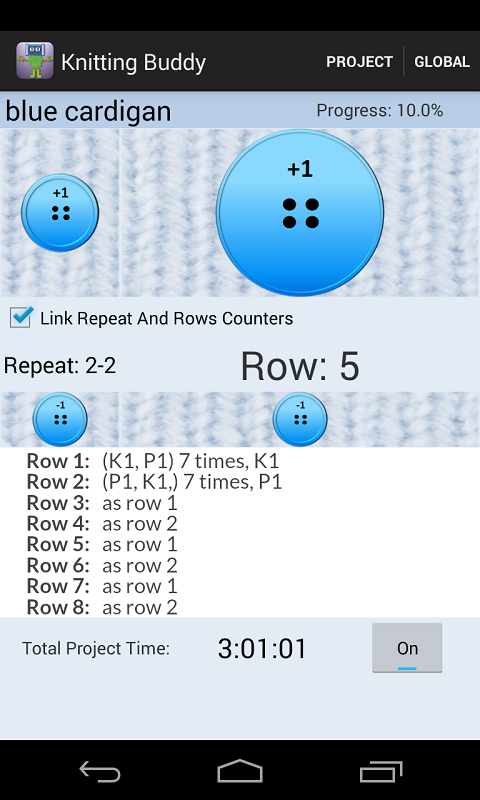
\includegraphics[width=2in]{images/image05.png}
  \caption[Counter of Knitting Buddy with chart picture \protect{\small at: \url{https://lh3.ggpht.com/KJfgkhsUvqPCJSxqd7TfO9gVRgivtng8nfHgUENAHx401J-EqgPvTbCMW-dTrWVqzJE=h900-rw} (last accessed: 2016-04-04)}]{Counter of Knitting Buddy with chart picture}
  \label{fig_knittingbuddy}
\end{minipage}
\end{figure}

\subsubsection{BeeCount knitting Counter by knirirr}
BeeCount differs from the standard of one row counter per project in that it allows multiple counters. Those counters can be for parts of the knit piece that  belong to the same project, as is the case for a knitted sweater, for example. These counters within a project can be linked together, so that increases or decreases in one counter affect the row number of another counter (figure 8). Furthermore, alerts can be set on counters to be triggered once the counter
reaches a set number.

\begin{figure}[H]
\centering
\begin{minipage}{.5\textwidth}
  \centering
  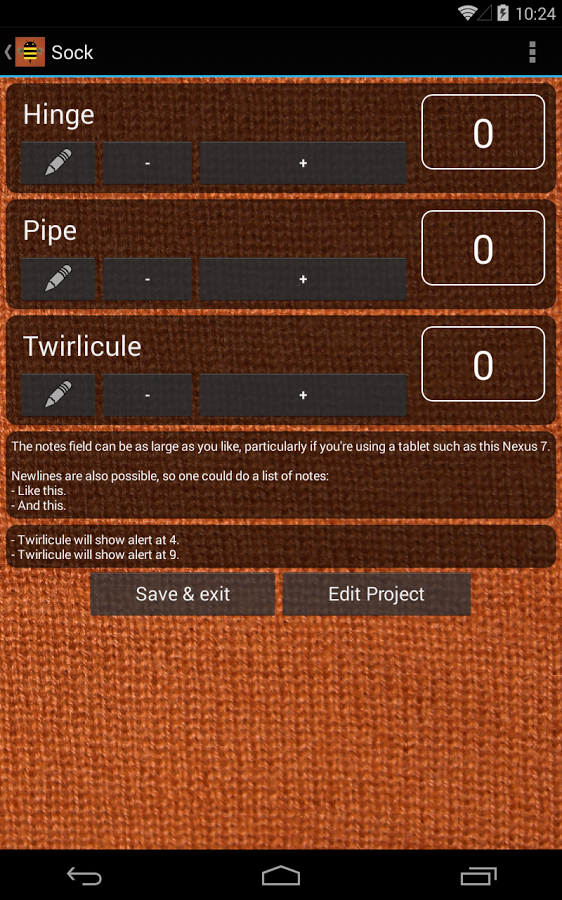
\includegraphics[width=2in]{images/image01.png}
  \caption[Counters of BeeCount \protect{\small at: \url{https://lh5.ggpht.com/CaLXmsrgU6JmB1iswLwffjY2eMfOgtt90H41RgHRmGPqro6XCrMdnkawc_TR4nhohYI=h900-rw} (last accessed: 2016-04-04)}]{COunters of BeeCount}
  \label{fig_beecount1}
\end{minipage}
\begin{minipage}{.5\textwidth}
  \centering
  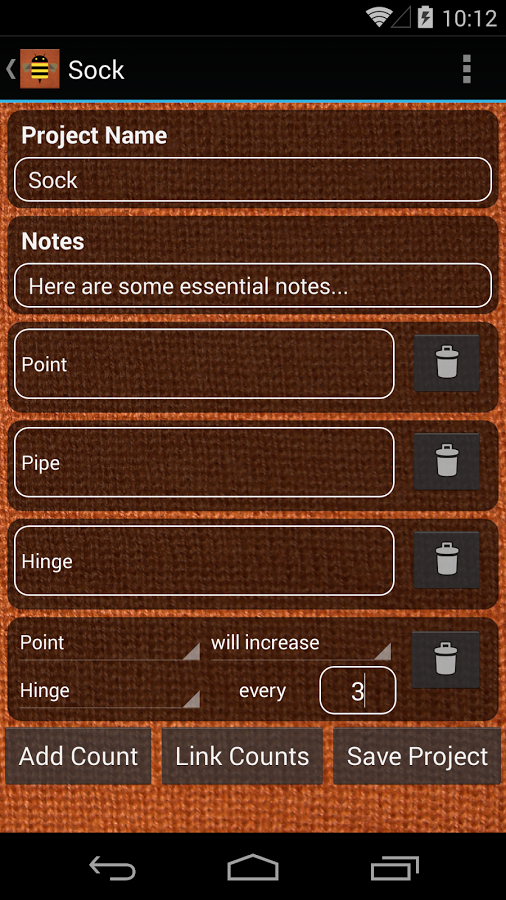
\includegraphics[width=2in]{images/image07.png}
  \caption[Counters set up of BeeCount \protect{\small at: \url{https://lh4.ggpht.com/ZD3ujRmMgBuxEaDjnCsc9fcN9k_kUQYwfEr_mQ23n7t-0sg-arQ0MMC-I52MI7ujc94=h900-rw} (last accessed: 2016-04-04)}]{Counters set up of BeeCount}
  \label{fig_beecount2}
\end{minipage}
\end{figure}


\subsubsection{Knitting Chart Maker by Awesome Applications}
When it comes to pattern charts, none of the aforementioned apps offers a solution besides the possibility to include a picture of a pattern. Therefore, I looked at Knitting Chart Maker, an app that focuses solely on the creation and editing of charts.

The app has over 30 stitch symbols that the user can use to create a pattern hart. The symbols are defined by the app and are not taken from a standard. The user can’t devise their own stitch symbols. Symbols can be used by selecting the symbol in the left-hand menu and then transferred onto the grid by tapping on a cell. Alternatively, the user can select the paintbrush button on the top-left menu and use their finger to paint the symbols onto every cell touched in a swiping motion, not unlike drawing with a pencil. The whole grid is zoomable up to a certain zoom level.

While in-app, the user can purchase the pro version which allows them to save and export patterns. Charts can be exported in the form of written instructions or a picture. Included are also various sharing features, such as uploading the saved chart to Dropbox, or sharing a chart with a friend, who can then open that chart in their paid copy of the app.

The app is locked in landscape mode and the chart dimensions are limited to 50 x 50. The pattern chart grid is implemented using OpenGl’s canvas and drawing images at the cell positions.

\begin{figure}[H]
  \begin{center}
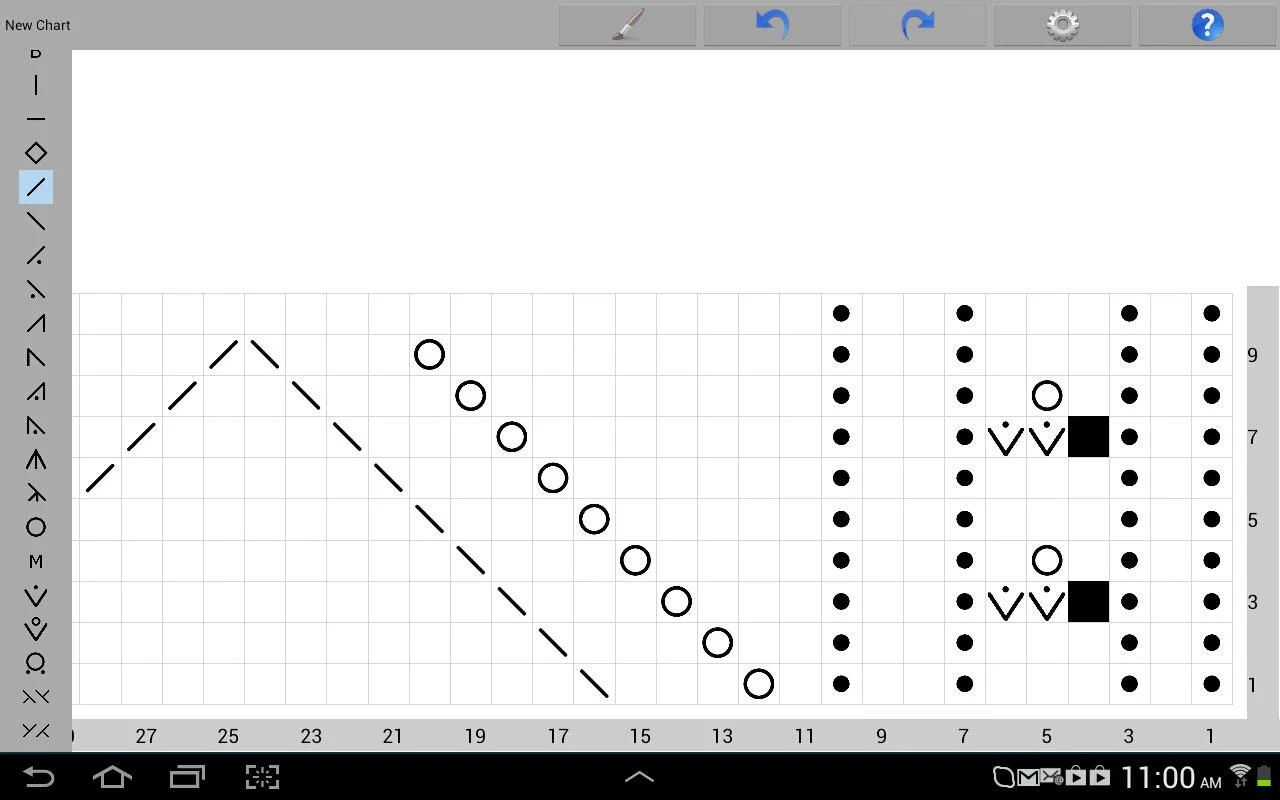
\includegraphics[width=2in]{images/image03.png}
\caption[Chart editor of Knitting Chart Maker \protect{\small at: \url{https://lh6.ggpht.com/MGKM0ukCDlMWWuboyxmZT-y8P3fTha4SI6l7u31eK3jFIkLsALlNEA_g6NffaoKRqyg=h900-rw} (last accessed: 2016-04-04)}]{Chart editor of Knitting Chart Maker}
\label{fig_knittingchartmaker}
\end{center}
\end{figure}

\subsection{Other}

\subsubsection{KnitML by Jonathan Whitall}
KnitML is an XML based format for describing the knitting process from beginning to the finished product. With KnitML The project aims to establish an international standard for knitting pattern expression\footnote{\url{http://www.knitml.com/blog/static.php?page=about-knitml}}. He aims to do so by using the Knitting Expression Langauge, KEL, that he defined (\cite{knitml}). KEL is based on the Groovy programming language\footnote{\url{http://groovy-lang.org/templating.html}} for the Java platform and the GroovyMarkup architecture.

The following KEL expression

\begin{lstlisting}[language=Java, caption=Example expression in KnitML]
Pattern {
    generalInformation
}
\end{lstlisting}

would result in

\begin{lstlisting}[language=XML, caption=Example expression in KnitM: XML result]
<pattern>
    <general-information/>
</pattern>
\end{lstlisting}

The project has not seen updates in any form since 2013 and I presume it discontinued. A beta of an editor program for KEL and its resulting XML can be found on the homepage of the project, knitml.com.

\chapter{Requirements}
\section{Functional Requirements}

The requirements for this thesis are formed from interviews conducted with volunteers at the beginning of this thesis. Three participants, stemming from both the author's acquaintances as well as from volunteers recruited from a poster posted publicly nearby the HTW’s campuses, have been interviewed. Prerequisite for a participant in such an interview was a proficiency and an interest in knitting. During a time frame of 45 to 60 minutes the participants were asked to answer a set of questions concerning their knitting experience as well as what features they would like to see in an app aimed to aid them during the creation and viewing of a knitting pattern chart. The catalogue of the questions asked and the answers given by the participants during these interviews can be found in the appendix \ref{appendix_user_interviews}. 
From these interviews user stories were formulated and corresponding functional requirements were extracted --- see table \ref{tabl:requirements}  below.

\label{tabl:requirements}
\begin{longtable}{| c | p{6.5cm} | p{6.5cm} |}
    \hline
   	\# & User Story & Functional Requirement \\ \hline
   	\endhead
    1 &	As a knitter I want to be able to see the knitting pattern chart on my phone while knitting &
	 Display of knitting pattern chart that is usable while knitting \\ \hline
	2 & As a knitter I want to create my own charts in the app both in a grid format and a row format & Create patterns that support row and grid format \\ \hline
	3 & As a knitter I want to transcribe charts from paper into the app with both grid and row formats & Pattern editor \\ \hline
	4 & As a knitter I want to have a list of all the patterns in the app and add and remove patterns from that list & \gls{crud} for patterns and showing list of patterns \\ \hline
	5 & As a knitter I want to convert metric units for needle sizes, yarn weight and length to imperial and vice versa & Unit converter in app  \\ \hline
	6 & As a knitter I would like to enter a set of written knitting instructions and be able to see each individual instruction while knitting and jump to the next instruction with a button press & Editor for written instructions and view of them to be used while knitting with button or voice command \\ \hline
	7 & As a knitter I want to use my phone to count the rows I knit & Row counter \\ \hline
	8 & As a knitter I would like to be able to look up the explanations and visual instructions for different kinds of stitches while inside the app & Glossary of stitches with explanations and instructions \\ \hline
	9 & As a knitter I want to have a way to jump to the row I'm currently on in my knitting pattern and to get back to the default zoom level & Button for resetting the zoom level and to jump to current row when viewing a pattern \\ \hline
	10 & As a knitter I want to be able to take pictures of the finished, knitted products of a pattern & In-app camera and function for adding images from disk \\ \hline
	11 & As a knitter I want to be able to see pictures of the knitted products of a pattern & Gallery for knitted products from a pattern \\ \hline
	12 & As a knitter I want to have all my knitting projects with their details (pattern, required needle size and yarn, etc.) easily accessible in one app & Knitting project management functions  \\ \hline
	13 & As a knitter I want to be able to use the row counter with another app in the foreground &  Have row counter increase and decrease button in notification bar when knitting app is not the active app \\ \hline
	14 & As a knitter I want my screen to stay on until I exit the app & Force screen to stay on while in-app \\ \hline
\end{longtable}

Within the context of this thesis the focus lies on the functional requirements \#1, 2, 3, 4, 7, and 8. The prototype of the app will present a functioning editor as well as a viewer for knitting pattern charts. Two input styles will be available for both viewer and editor: a grid style and a row style. The in-app generated pattern will be stored on disk and will be accessible with \gls{crud} operations within the app. The viewer will have a row counter next to the displayed pattern chart. Buttons for switching between the view styles will be present in the editor as well as the viewer. The option to import and export pattern files will be available as well in case the user wants to move their patterns to or from a different Android device. 

After these requirements have been fulfilled and if time allows, additional features for the app will be: a button for resetting the zoom level and jumping back to current line in the pattern, a row counter increase and decrease button outside of the app, and the option to force the screen to stay awake while within the app.

\section{Non-functional Requirements}

The prototype must have good usability and be robust, meaning it should be able to handle errors without crashing. Pattern files must be able to be backed up locally and be accessible by the user. All prototype functionalities will run locally, connectivity to the internet is not needed. Internet connectivity is an option for a later version of the prototype, e.g. for backing the pattern files up to cloud storage and sharing patterns. Since this thesis focuses on the \gls{UI} part of an app, storage will be restricted to simple, local solutions. This is also done to better fit the time restraints placed in this thesis. 

\chapter{Design}
The desired outcome of this thesis will be a working Android app prototype with working CRUD functions for knitting chart patterns and a row counter functionality while viewing a pattern. This prototype is intended as an aid for knitters of all backgrounds during their respective knitting projects. Patterns will be saved locally as a \gls{json} file on the device's internal storage. It would also be an option to store patterns on a server and let the app play the role of client, but that would not fit within the time constraints of this thesis. To give the user the ability to backup their patterns the app will support the import and export of pattern from external storage. For a detailed explanation of Android's concepts of internal and external storage see section \ref{storage}. Patterns exported will be accessible by the user and can be handled in whatever way the user sees fit to, for example, share or upload a pattern.

A chart pattern will consist of a set number of rows and columns. Each cell of the grid contains a symbol representing a knitting stitch. Created pattern are stored locally on the device and can be manipulated by the user in-app, as CRUD operations apply. Creating, editing and viewing patterns will be based on two shared visual formats for the pattern: a grid format and a row format.

The grid format will display the pattern in a grid, simulating the most common form of commercial distribution for knitting chart patterns on both analogue and digital media. Manipulation of the pattern content will be possible through a software keyboard containing the stitch symbols. A symbol can be selected and then applied to cells in the grid via touch. The symbol will stay active until the user selects a different symbol. The grid size can be changed with a button which opens a dialog where the desired amount of rows and columns can be entered. On confirmation the grid will shrink or expand to the set dimensions. Any symbols lying outside of the new bounds will be deleted, whereas new cells will be empty.

Similar to the grid format the row format will display the pattern rows, but will forego the representation of the columns. Instead the cells of a row will be summarized in such a way, that consecutive, identical symbols will be represented  by a number value equal to the count of the symbols and followed by the stitch symbol. Rows in this format can be edited like a conventional text editor - a movable cursor to show where further user input will be inserted and text selection functions for multiple character deletion, copying and pasting will be available. The software keyboard corresponding to this format will consist of the stitch symbols and a num pad, as well as an enter and a backspace key.

Viewing a pattern will come with a row counter below the actual chart pattern. This counter can be increased, decreased and reset by utilizing buttons. The counter is limited between one, as the first row of a pattern, and the number of rows the pattern contains in total. The current row will be indicated through a highlight on the pattern, marking the corresponding row in both grid and row format. When exiting the viewer the current row number will be saved in the pattern file and applied to the counter the next time the pattern is viewed

While editing or viewing a pattern, the row and the grid format will allow the user to 2D scroll, meaning both vertical and horizontal scroll. Additionally, the grid view can be zoomed and reset to default zoom and scroll. Switching between both formats while editing and viewing a pattern will be supported with a button. Upon switching the pattern will be saved. Renaming, deleting, saving, and exporting the pattern will be possible from within both formats with menu entries.

On app launch the list of patterns saved on the device will be shown. While viewing that list menu entries for exporting all patterns and importing a single pattern will be available. For the import the user can choose a file on the device from a file chooser. Exporting will export files to a set directory on the publicly accessible storage of the device. A list item will consist of the pattern name, an edit, and a delete button. A click on the pattern name will open the pattern in the viewer in row format with the default dimensions of 10 columns and 10 rows. Below the list will be a button to create a new pattern which will open a dialog for entering the new pattern’s name. After confirming a name, the editor will open with the row format.

\begin{figure}
  \centering
  \begin{minipage}{1\textwidth}
    \centering
    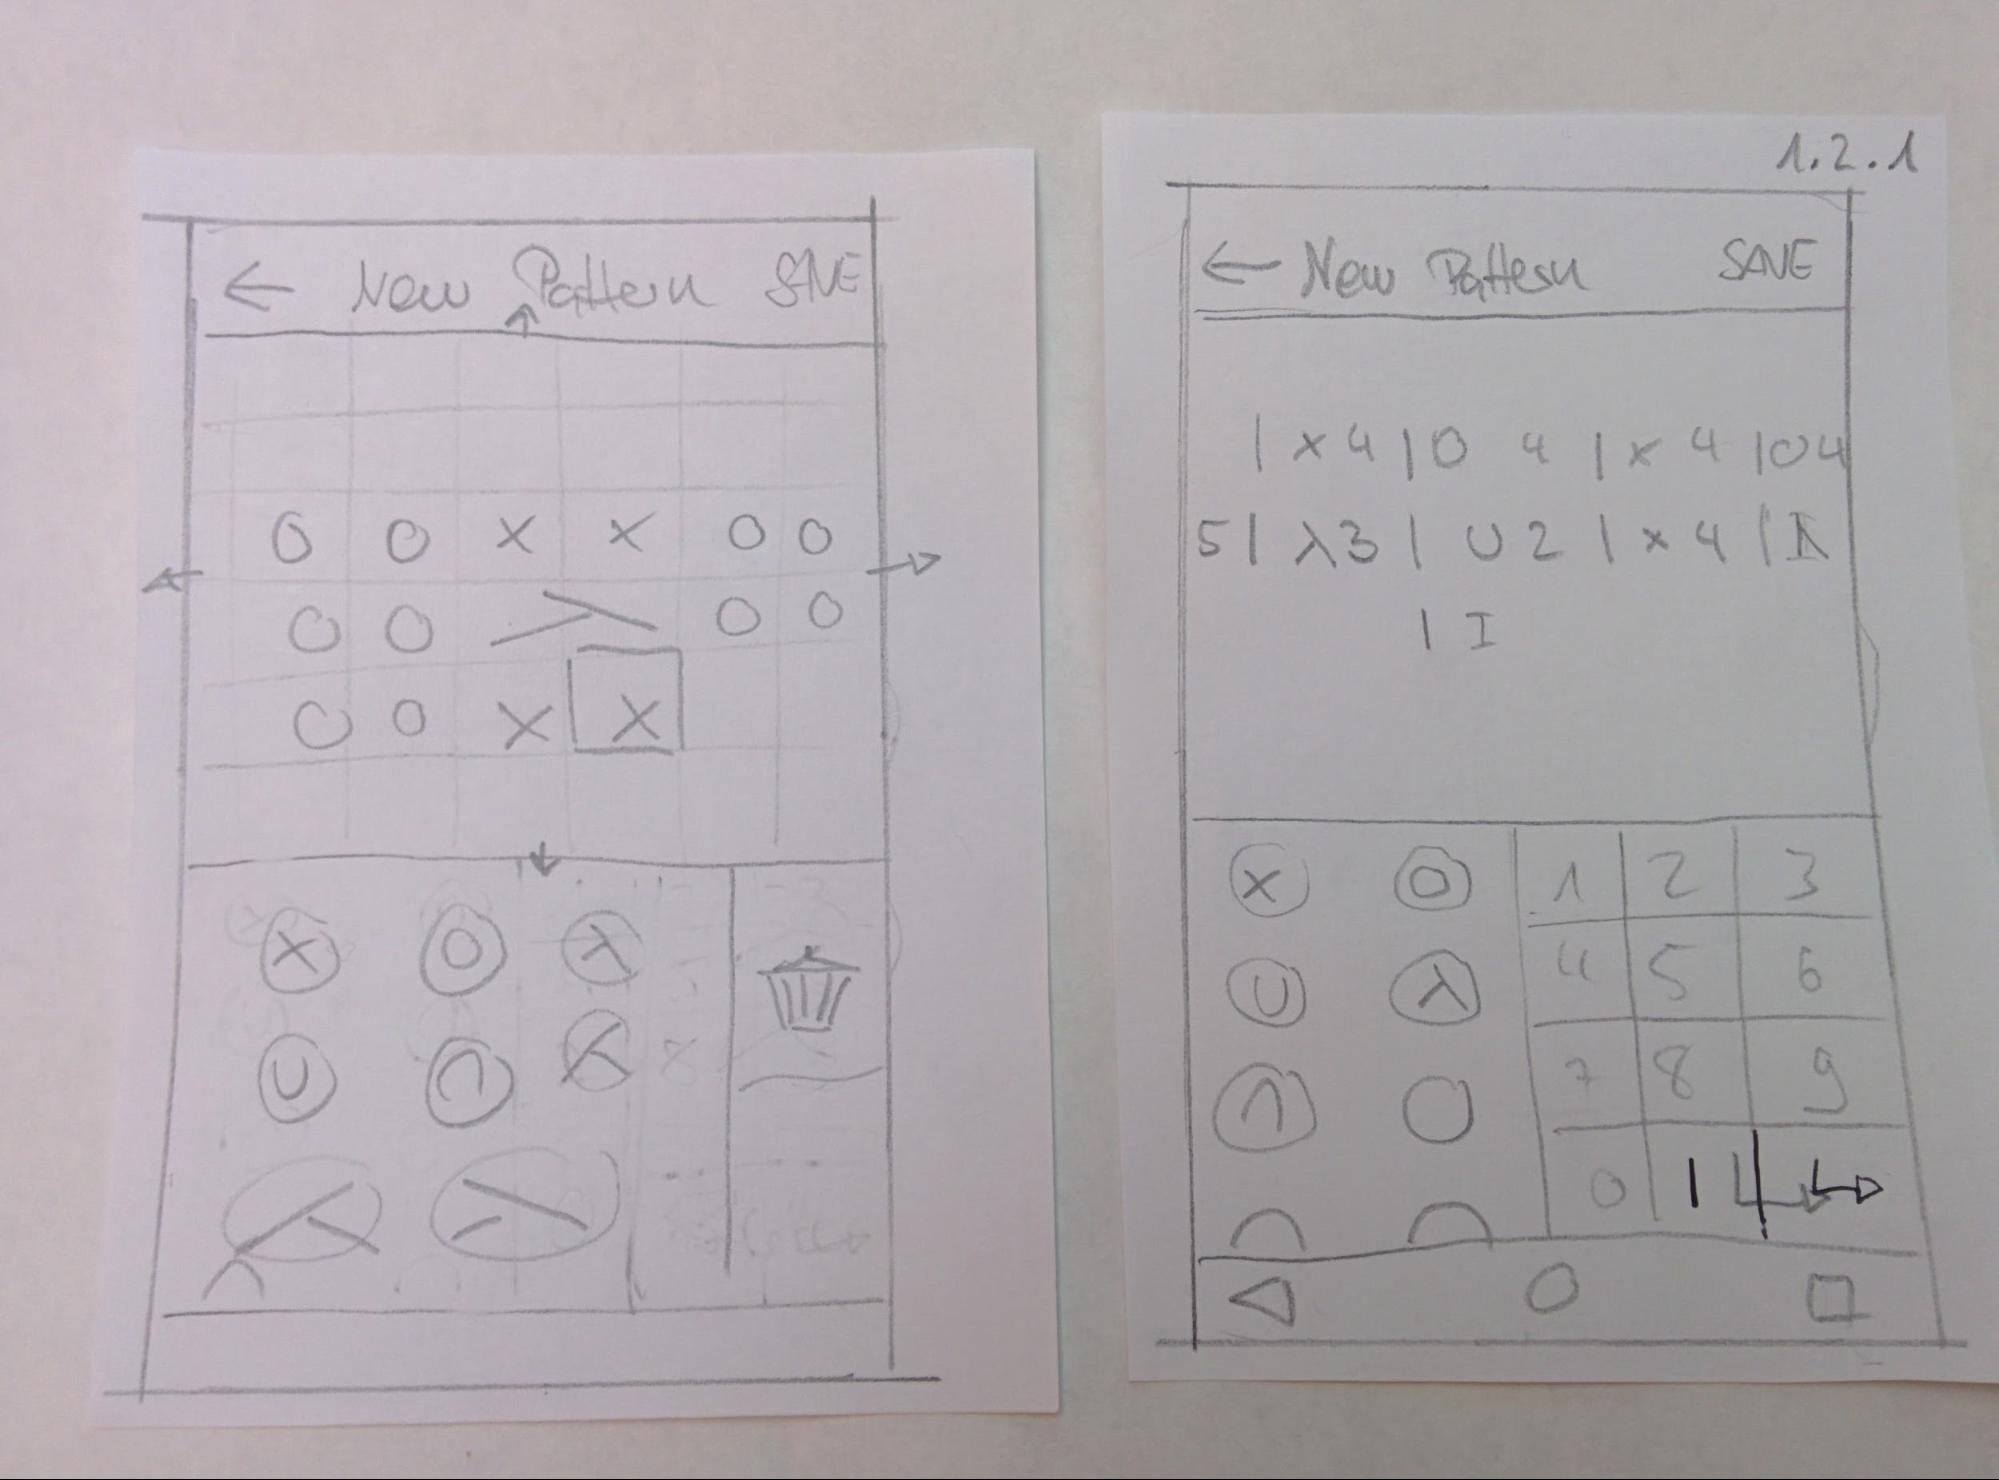
\includegraphics[width=1\linewidth]{images/image09.jpg}
    \caption{Editor screens for grid and row format with pattern name and save button in navigation bar}
    \label{fig_wireframe1}
  \end{minipage}

  \begin{minipage}{1\textwidth}
    \centering
    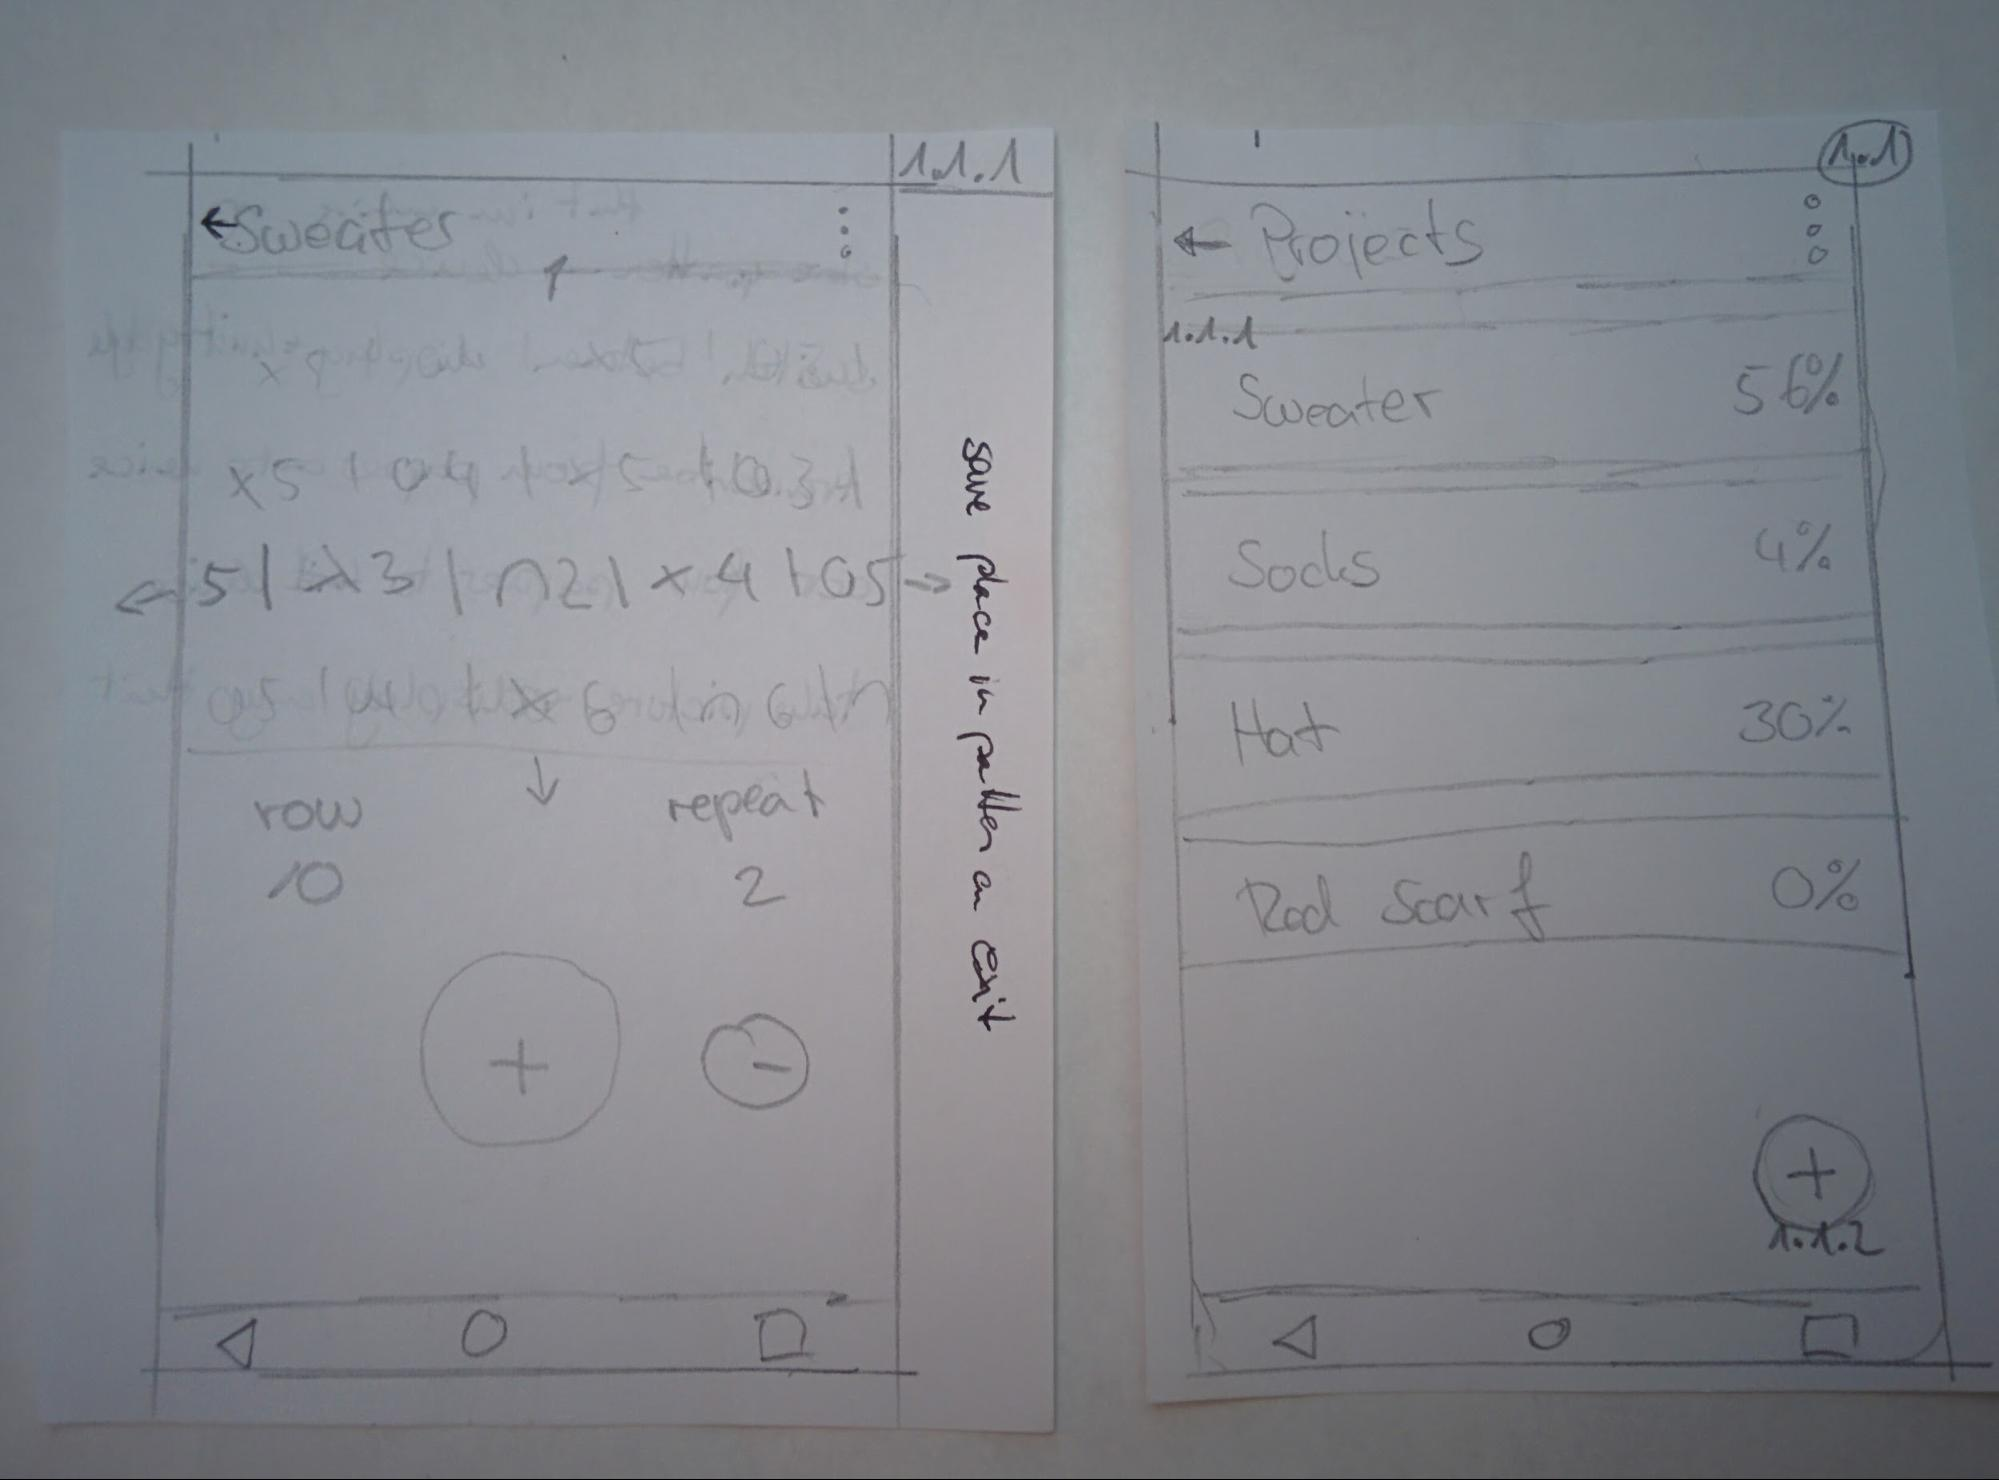
\includegraphics[width=1\linewidth]{images/image08.jpg}
    \caption{Viewer screen for row format and selection screen for stored patterns}
    \label{fig_wireframe2}
  \end{minipage}

  \caption{Screens for editor and viewer without Android elements}
\end{figure}

\begin{figure}
\centering
\begin{minipage}{1\textwidth}
  \centering
  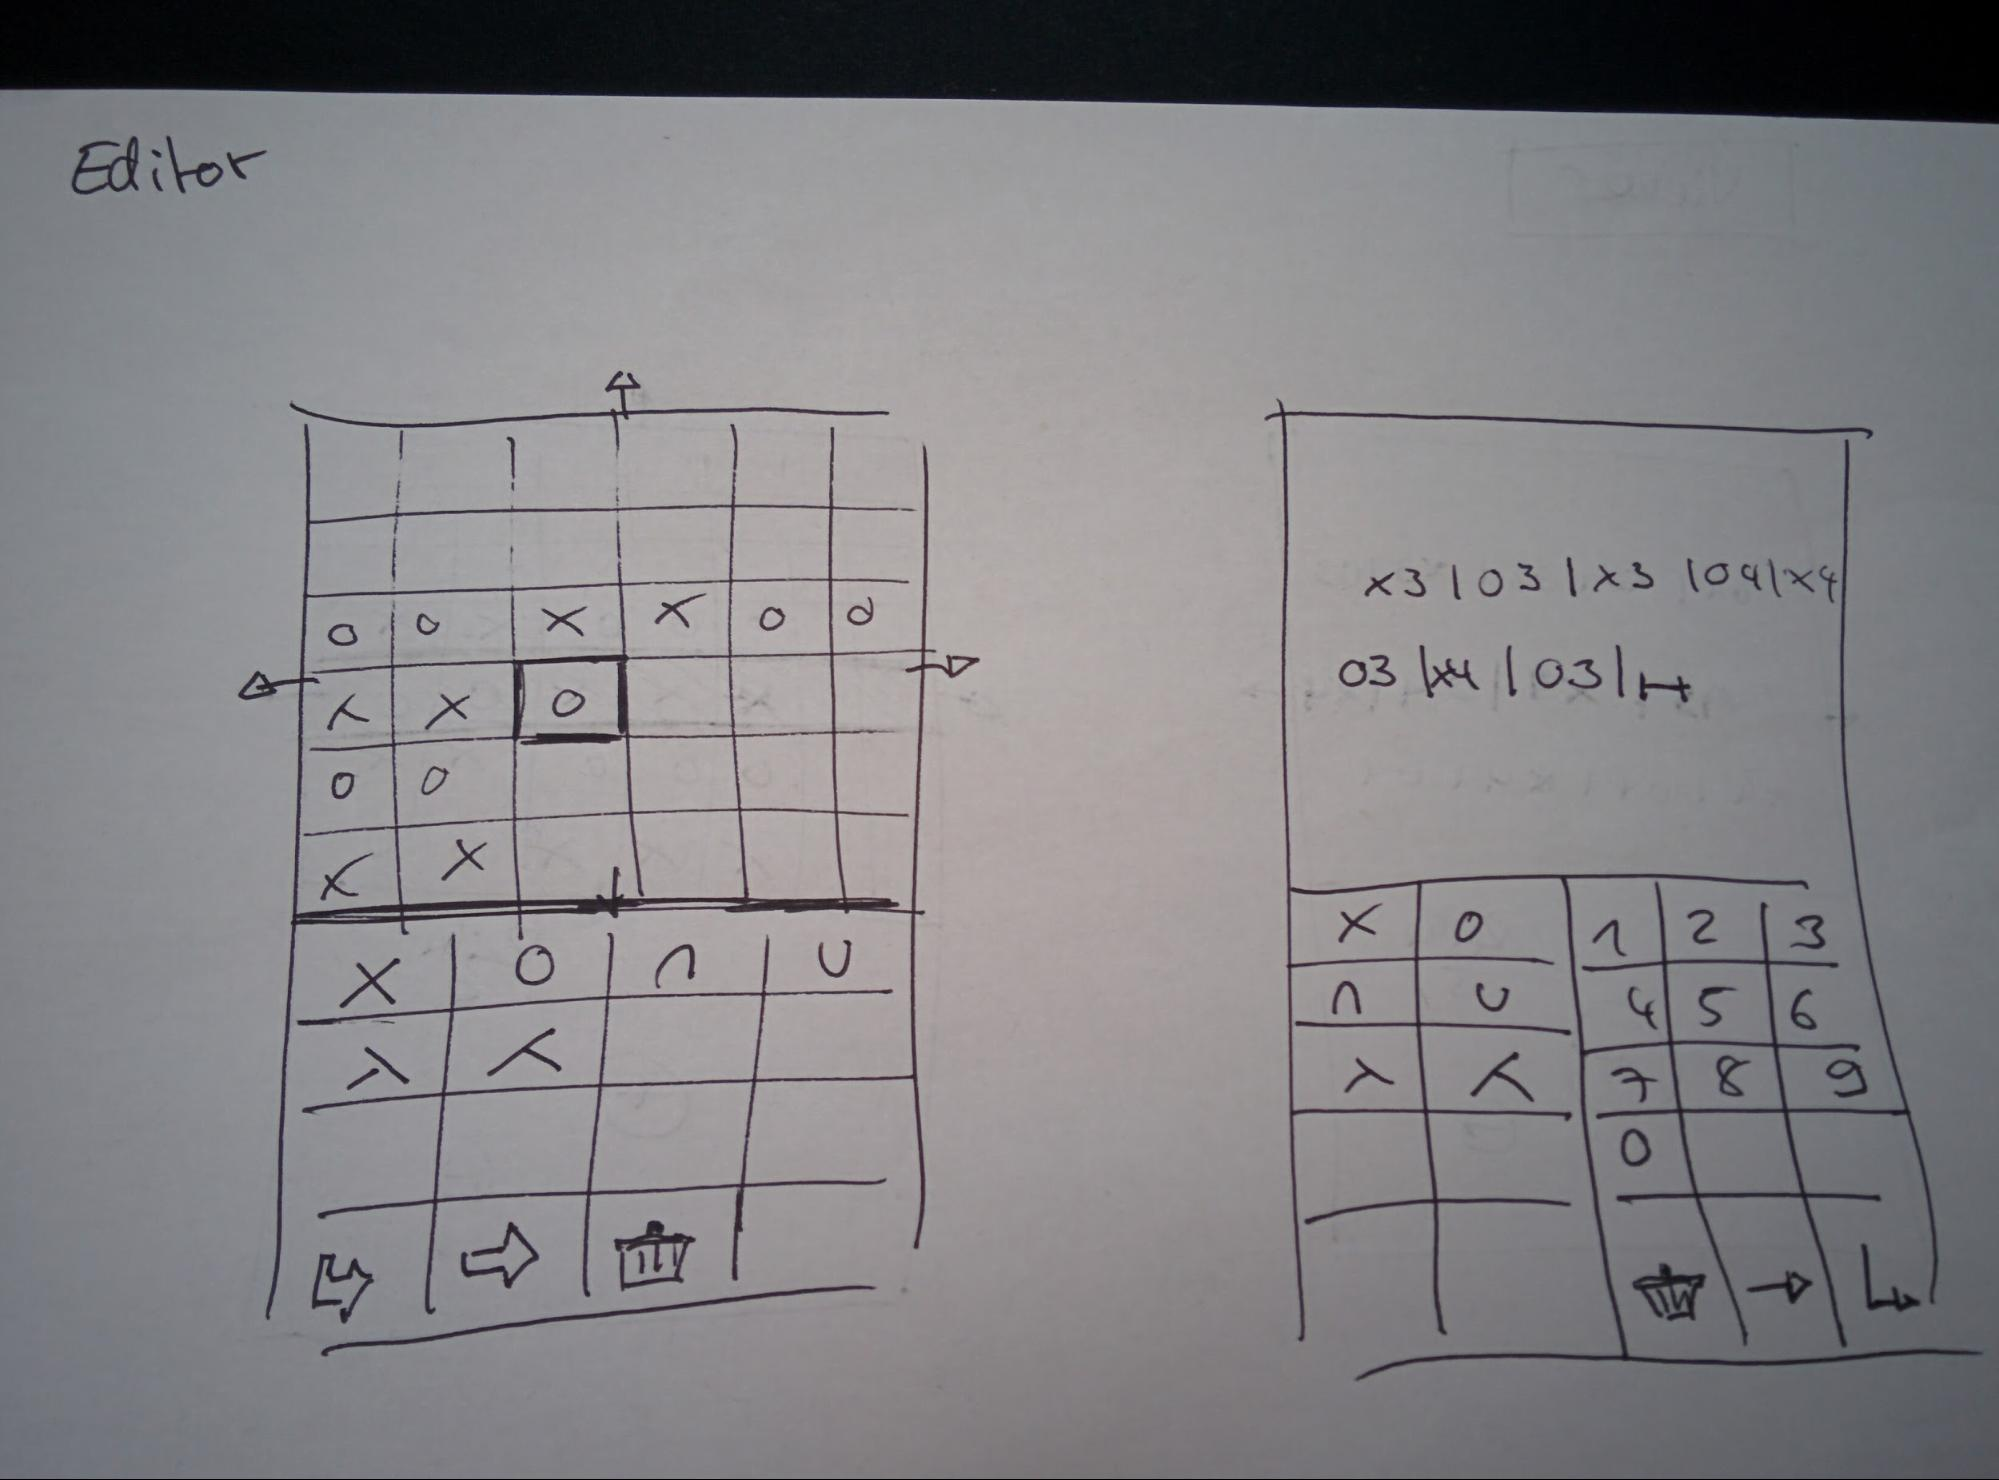
\includegraphics[width=1\linewidth]{images/image00.jpg}
  \caption{Editor screens for grid and row format}
  \label{fig_wireframe3}
\end{minipage}

\begin{minipage}{1\textwidth}
  \centering
  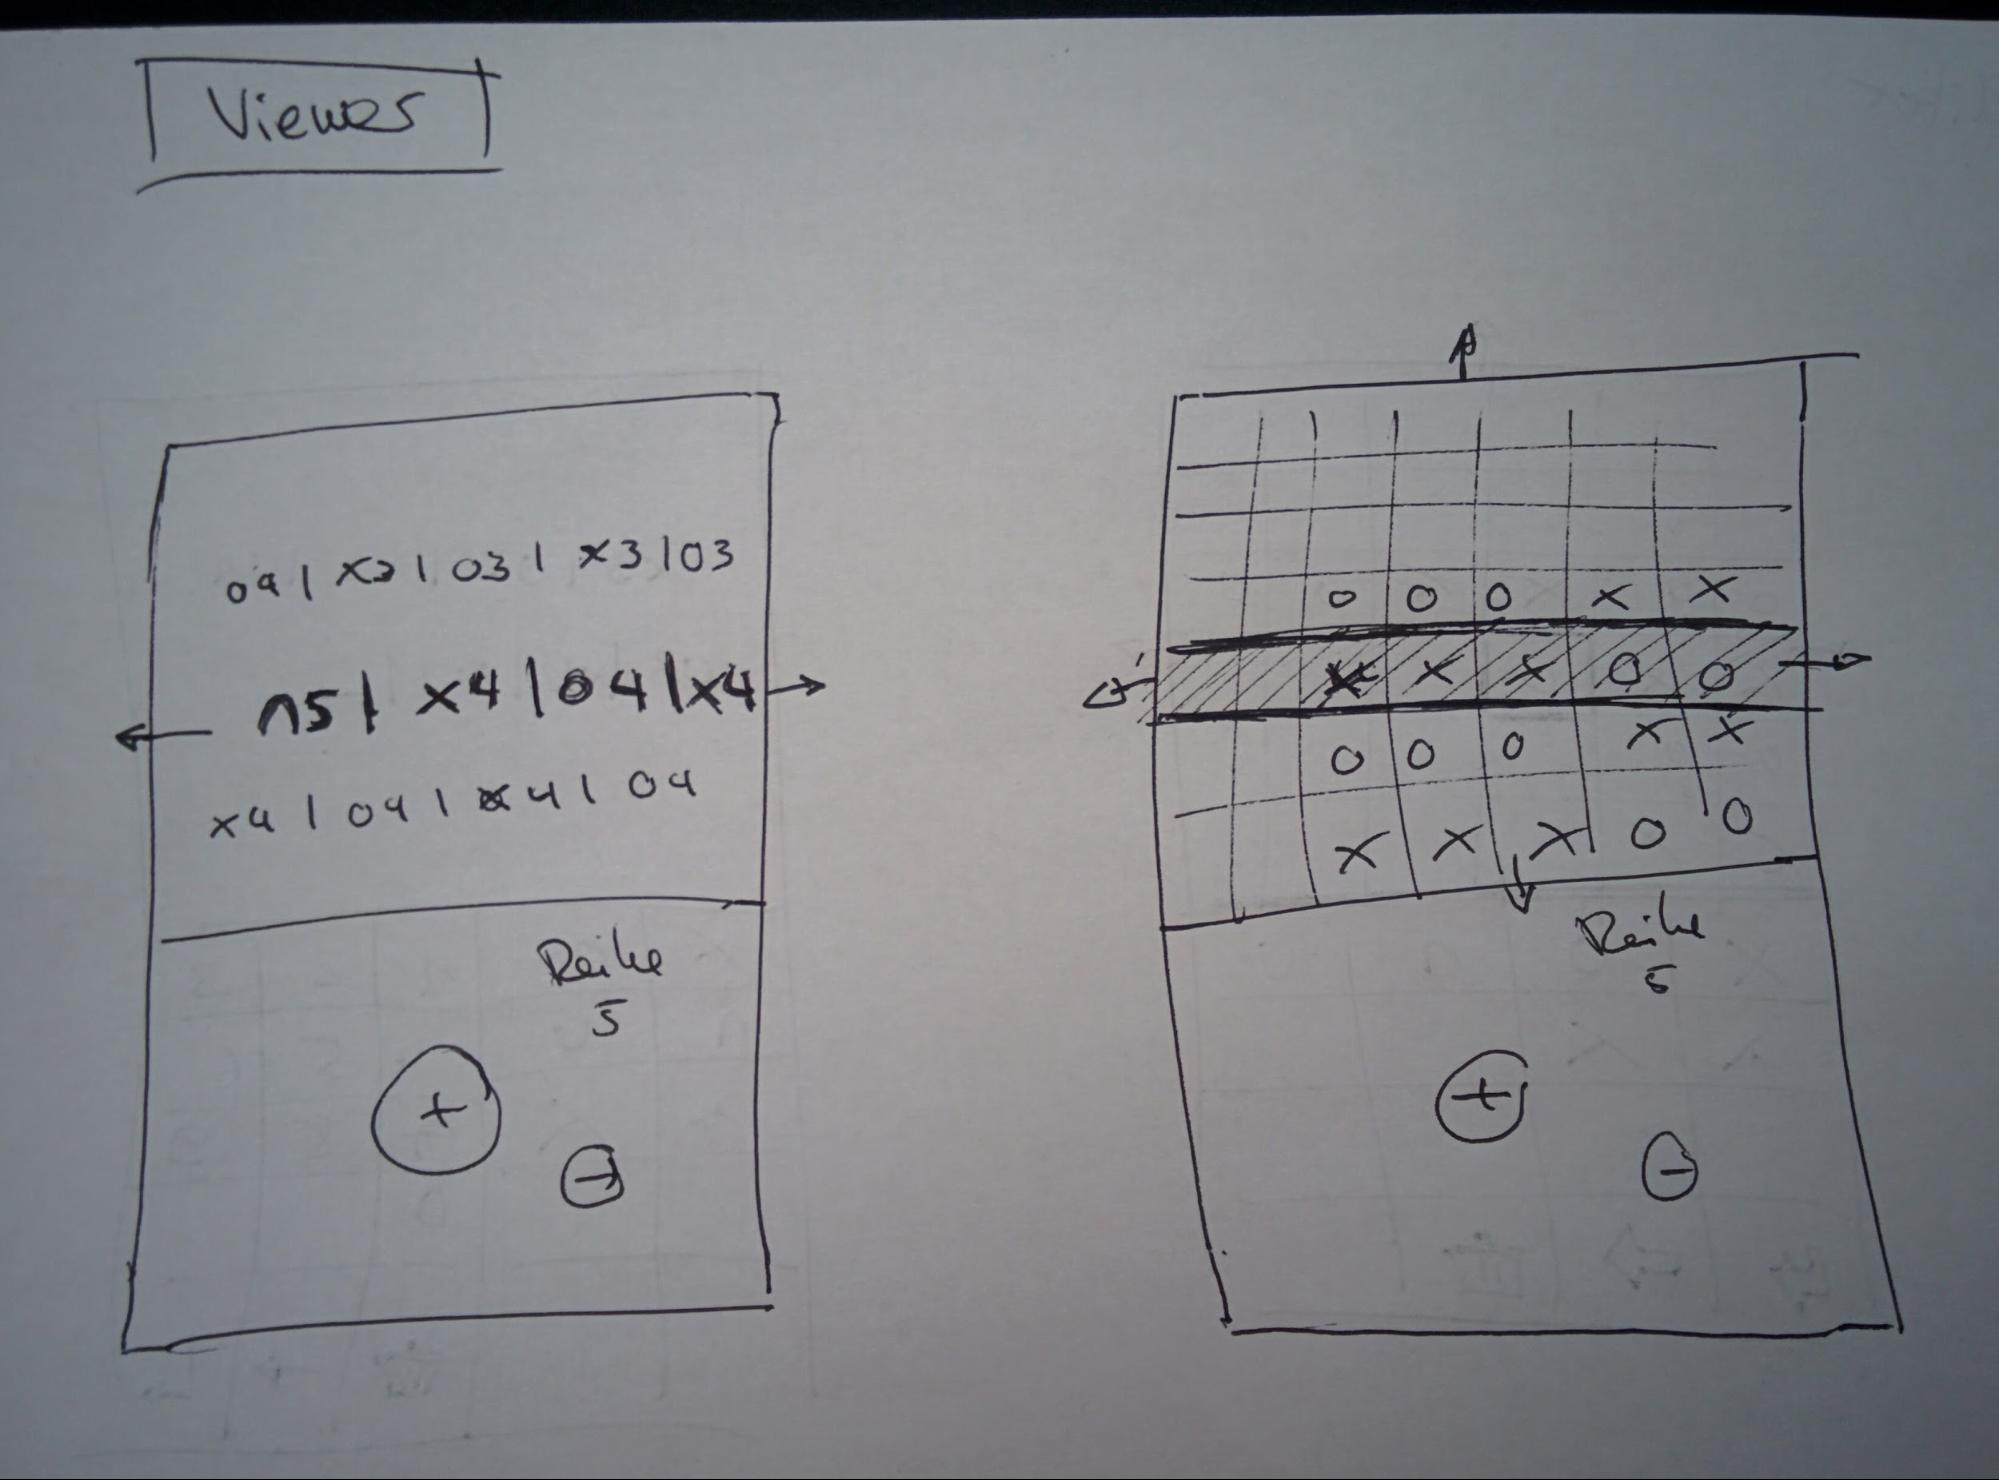
\includegraphics[width=1\linewidth]{images/image02.jpg}
  \caption{Viewer screens for grid and editor format with row counter}
  \label{fig_wireframe4}
\end{minipage}
\end{figure}

\chapter{Android Basics}
\section{The Operating System Android}
Android is an open source operating system for mobile phones and tablets based on the Linux kernel (\cite{androiddef}). Android apps are distributed on Google Play, a service owned by Google. To build an Android app Google offers the Android \gls{SDK}, containing sample projects, necessary Android libraries and an Android emulator. Additionally, Google recommends to use the official Android \gls{IDE} Android Studio, which is based on IntelliJ IDEA and offers many useful tools, including testing frameworks, a \gls{GUI} for screen layouts, and the build tool Gradle (\cite{androidstudio}). The concepts and Android components discussed throughout this chapter are taken from the Android Developer reference\footnote{\url{https://developer.android.com/reference/packages.html} (last accessed 2016-08-11)}, training\footnote{\url{https://developer.android.com/training/index.html} (last accessed 2016-08-11)}, and \gls{API} guides\footnote{\url{https://developer.android.com/guide/index.html} (last accessed 2016-08-11)} found online.

\section{Basic Components of an Android App}

\subsection{Activity}
The \code{Activity} class is needed to display any user interface and as such usually has a single purpose --- handling a login would be such a purpose. An app consists of one or more activities that are in some way connected to each other (\cite{activities_in_app}). \code{ViewGroups} and \code{Views} can be added to the view hierarchy of activities and fragments (see Section\ref{impl:fragment}) --- these views define different UI components for Android. An activity can also embed multiple fragments which then live in a viewgroup inside the activity's own view hierarchy (\cite{androidfragment}). When containing fragments, the activity’s job is that of managing those fragments through getters and setters and orchestrating the communication between fragments, which is done with callbacks defined in the fragments. 
An activity features methods such as \code{onCreate()}, \code{onStart()}, \code{onStop()}, and \code{onFinish()}, which can be overwritten to implement logic that is executed at different points in the activity's lifecycle (see \reffigure{fig:activity_lifecycle}). The same applies for a fragment, but where an activity can stand alone, a fragment always needs to be attached to an activity; it is connected to that activity's lifecycle.

\begin{figure}[H]
  \centering
    \begin{subfigure}[b]{0.6\textwidth}
      \centering
      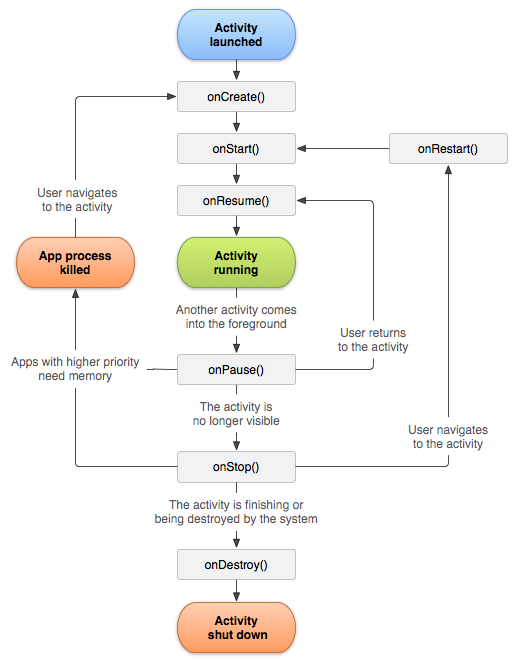
\includegraphics[width=\linewidth]{images/activity_lifecycle.png}
      \caption[{The lifecycle of an activity \protect\newline{\small at \url{https://developer.android.com/images/activity_lifecycle.png} (last accessed: 2016-04-04)}}]{The lifecycle of an activity}
   \label{fig:activity_lifecycle}
    \end{subfigure}
    \begin{subfigure}[b]{0.3\textwidth}
      \centering
      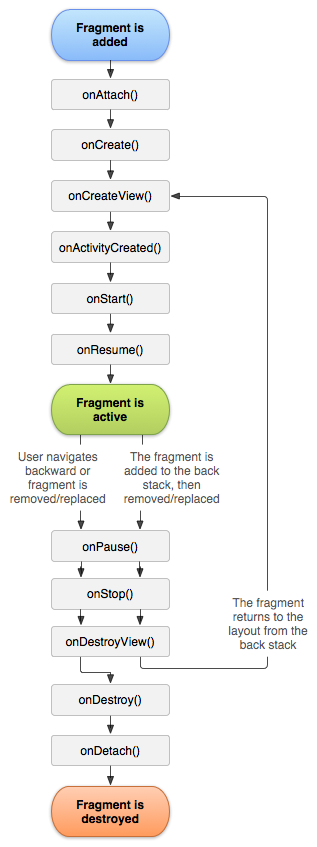
\includegraphics[width=\linewidth]{images/fragment_lifecycle.png}
      \caption[The lifecycle of a fragment \protect\newline{\small at: \url{https://developer.android.com/images/fragment_lifecycle.png} (last accessed: 2016-08-09)}]{The lifecycle of a fragment}
    \label{fig:fragment_lifecycle}
    \end{subfigure}
  \caption{The lifecycles of activities and fragments}
\end{figure}

\subsection{Actionbar}
The \code{ActionBar} located at the top of an app and has several important functions. It displays the application name or the title of an activity, houses the action buttons, and the action overflow. Action buttons should contain the most common and important actions used in an app (\cite{actionbar}). The action overflow contains action buttons that are hidden from plain view, either because the actionbar was not wide enough to show all buttons or because of a deliberate design decision. Such a decision is usually made when the button in question is connected to an action that is rarely used, e.g. renaming something, or when the action has far-reaching consequences and shouldn't be near buttons that are used frequently, lest the user accidently hits it. Such an action could be the deletion of the pattern currently being edited, such as in the case of a knitting app. 

\subsection{Fragment}
\label{impl:fragment}
The \code{Fragment} class usually implements a specific user interface or behaviour and should, ideally, be modular, so that they can be reused within multiple activities or in different screen configurations. Just like an activity a fragment has its own lifecycle, see \reffigure{fig:fragment_lifecycle}.

A fragment's creation is always embedded in an activity (\cite{androidfragment}) --- forcing the fragment to pause or stop alongside its parent activity's lifecycle. Fragments can also house viewgroups and views and are intented to function as interchangeable modules, e.g. as \gls{UI} modules for an app that runs on devices of varying sizes and that wants to present the user with a dynamic \gls{UI} fit to suit the screen size (see \reffigure{fig:fragments_uimodules}). Android offers different fragment subclassse with predefined behavior, such as the DialogFragment class, that opens a fragment as a floating dialog by default (see \reffigure{fig:fragment_dialog}).

\begin{figure}[h]
  \centering
    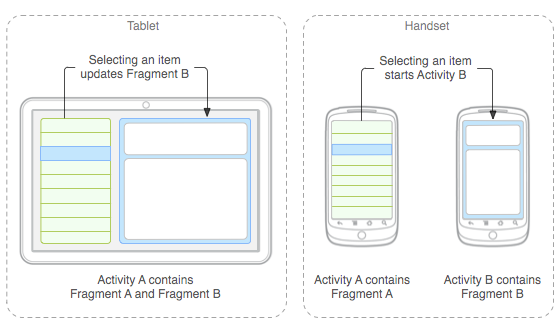
\includegraphics[width=.7\textwidth]{images/fragments.png}
   \caption[Two fragments of one activity and their layout on two different screen sizes. \protect\newline{\small at: \url{https://developer.android.com/images/fundamentals/fragments.png} (last accessed: 2016-08-09)}]{Two fragments of one activity and their layout on two different screen sizes} 
    \label{fig:fragments_uimodules} 
\end{figure}

\begin{figure}[H]
  \centering
  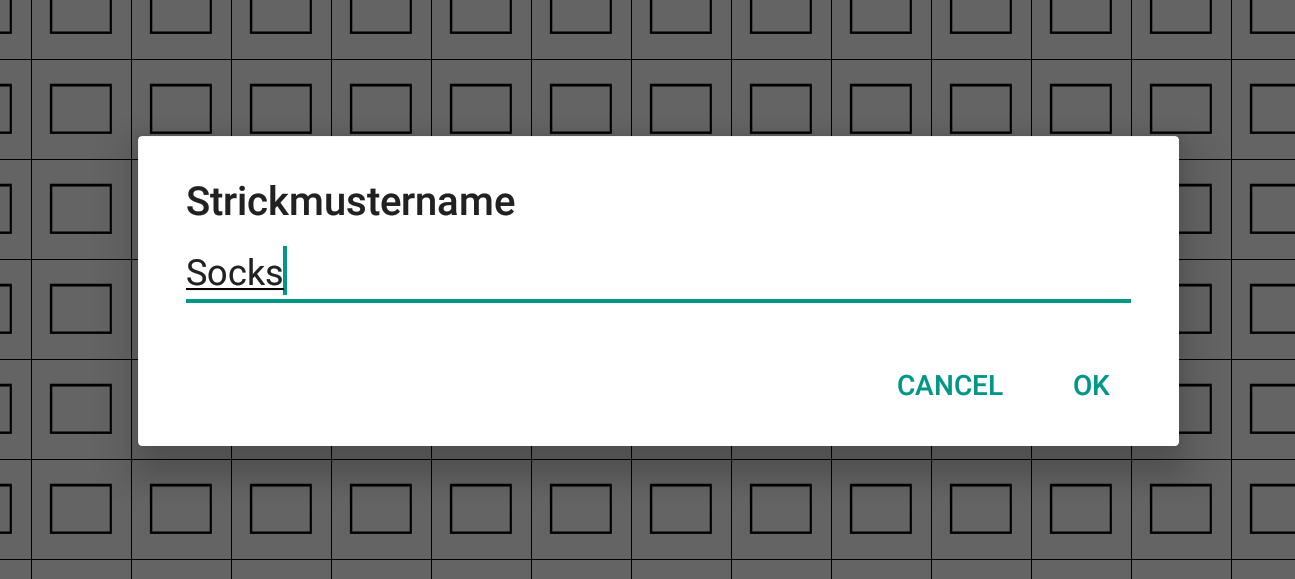
\includegraphics[width=.7\textwidth]{images/pattern_name_dialog.png}
  \caption[A dialog fragment for naming a pattern \protect\newline{\small (own image)}]{A dialog fragment for naming a pattern} 
  \label{fig:fragment_dialog} 
\end{figure}

Communication between different fragments needs to be handled by the activity, which manages the fragments. An activity communicates with a fragment by keeping a reference to the fragment and calling its public methods. On the other hand the fragment should not possess a reference to its parent activity --- instead the parent activity should implement a callback interface defined inside the fragment (\cite{fragment_event_callback}). A good practice to enforce the implementation of a fragments callback interface is to check for its existence when the fragment is attached to the activity --- example code proposed by the Android Developer guide concerning how to check for this can be seen in \reflisting{lst:callback_interface} (\cite{fragment_event_callback}).

\vspace*{0.5cm}
\begin{lstlisting}[language=JAVA, caption=Example code for enforcing the implementation of a callback interface, label=lst:callback_interface]
public static class FragmentA extends ListFragment {
    OnArticleSelectedListener mListener;
    ...
    @Override
    public void onAttach(Activity activity) {
        super.onAttach(activity);
        try {
            mListener = (OnArticleSelectedListener) activity;
        } catch (ClassCastException e) {
            throw new ClassCastException(activity.toString() + " must implement OnArticleSelectedListener");
        }
    }
    ...
}
\end{lstlisting}

\subsection{View}
Views are the most basic block that the \gls{UI} is built from (\cite{android_view}). A view's bounds are always rectangular and its position is defined by its top and left coordinates with the point of origin at the top left. It is the view's job to handle its drawing and event handling. For this the view has the predefined methods \code{onDraw()} and \code{onTouchEvent()}, respectively. The \code{View} class is also the base for viewgroups which in turn are the base for layouts, containers for other views or viewgroups.
The views from a window are arranged in a tree structure. Views can be added to this tree statically, by specifying them in a \gls{XML} layout file, or dynamically, from code. Android comes with plenty of view subclasses, specialized in acting as controls or displaying specific types of content, e.g. text or images. If the pre-existing views don't match a developer's needs, they can also implement a custom view to take control of the drawing and the event handling as it fits their requirements. For this the \code{onDraw()} method can be overridden and custom operations can then be executed on the \code{Canvas} object that is contained in the method parameters.

Android ships with many subclasses of View, e.g. the \code{TextView} class which diplays text content. The view class is also the basis for viewgroups, to which the layouts, e.g. \code{LinearLayout} and \code{RelativeLayout}, belong to. Views in a window are bundled together as a tree hierarchy with a layout being the top-most root. To add views to an activity or fragment the views can be declared in the corresponding \gls{XML} layout or from code. 

\subsection{Storage}
\label{android_storage}
File storage in Android devices is separated into ``internal'' and ``external'' storage --- this refers to Android devices often having a built-in, non-removable memory and an external, removable medium in the form of an SD or a micro SD card (\cite{android_storage}). This storage separation even exists on devices with only built-in memory --- in such cases the storage is partitioned into ``internal'' and ``external'' partitions. This assures that the concept of two storages persists across all devices and \gls{API} levels. The internal storage is inaccessible by the user under normal circumstances --- exception to that is when the user has root privileges, e.g. on a rooted phone. This storage houses, among other things, files from apps, e.g. databases. These files are only accessible by the app that originially places them in the interal storage --- neither user nor other apps can access them. Files are removed when the app they belong to is uninstalled. 
The external storage on the other hand is more public. Files placed here can be read and written by the user as well as other apps and they remain even after the app they orignated from is uninstalled. When working with the external storage it is important to check that it is not currently used as \gls{USB} storage by a computer the device is connected to.
Apps have by default read and write access to the directory they are installed in on the internal storage, but to access the external storage the app requires that the user grants the app a specific permission. This permission needs to be declared in the app's manifest file, an \gls{XML} file that every app must have. This file contains information required by the Android system to allow the app to run, such as the activities contained in the app and the permissions the app requires.

Beginning in Android 6.0 (\gls{API} level 23) apps targeting that version need to request and aquire dangerous permissions at run time (\cite{android_permissions}), whereas before the app was given all permissions listed in its manifest upon agreeing to a dialog popup when installing the app. Dangerous permissions cover access to the user's private data or to affect areas where the user stores their data or data that other belong to other apps (\cite{android_permissions}). Since the user can revoke permissions for apps at any given time the developer needs to take extra steps to keep the app running even when some features need to be disabled because of missing permissions.  


\chapter{Implementation}
\textit{Google’s IDE Android Studio 2.1.2 was used for the implementation of the Android app prototype targeting Android 6.0 Marshmallow (\gls{API} level 23).} 

\section{Stitch symbols}
There are different ways to display a stitch symbol in an Android app --- this section will give an overview of the possibilities and the solution chosen for the prototype. 
Since the \code{View} class already defines a canvas object with dedicated functions for drawing image and text content in its \code{onDraw()} method, it offers a good starting point. To decide between using the image or text format for displaying stitch symbols, a further look into what each format entails is necessary.

Image content needs to be specified in an Android project in the res directory under the drawable directory. This directory contains the image resources of the app, the drawables --- this applies for icons, custom images, and other image content, excempting the launcher icon of the app, which is located in the mipmap directory. One way to use stitch symbols in an Android app would be to add every symbol as a drawable resource, and then draw those resources to the canvas of a view. For this a drawable would be needed for each individual stitch symbol, as well as way to map these drawable files to values that can be efficiently stored in a \gls{json} file. The usage of many drawables in an app would also lead to an increase in app size, resulting in longer download times and larger storage demands. Both are an inconvenience to the user and can be problematic on older devices with less powerful hardware, making the app unsusable in the worst case scenario.
The other option for displaying symbols is to create a custom \gls{TTF} with glyphs for stitch symbols that is applied to text in the app. This is the solution used in the prototype. It offers several advantages over using image resources. For one, when using drawables it might be necessary to include several versions of the same file to ensure that they are displayed correctly on devices with different screen densities (\cite{android_screen_densities}). This is not needed for text with a custom font: the glyphs are defined by Beziér curves, which are correctly rendered by the system for the individual screen densities. The usage of a font also allows to write each stitch as a character, simplifying the process of saving a pattern to a \gls{json} file. For OpenType fonts, which \gls{TTF} belongs to, Microsoft recommends 64000 as the maximum number of glyphs a font should contain (\cite{microsoft_max_glyphs}). This allows for a plethora of stitch symbols. There are several knitting fonts available online, e.g. the Kauri Knits font by \cite{kauri} and the Knitter's Symbol font by \cite{xenakis}. To ensure that the knitting symbol glyphs fit within the style of the grid and row format an example of a custom knitting font was created for this thesis by the author.

The open source program FontForge \footnote{\url{https://fontforge.github.io/en-US/} (last accessed: 08-10-2016)} was used creation of the custom \gls{TTF} knitting font used in the protoype. The knitting font contains a selection of 16 stitch symbols whose glyphs were defined by the author herself. The glyphs and their corresponding UTF-8 characters can seen in \reffigure{fig:own_knitting_font}. The available symbols the knitting font offers as well as the corresponding symbol descriptions need to be defined as string arrays in the Constants class in the project.

\begin{figure}[H]
  \centering
  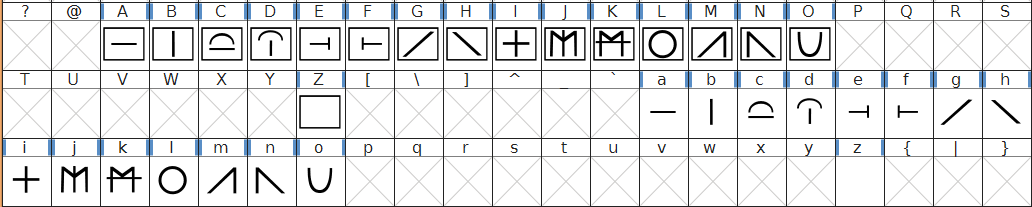
\includegraphics[width=.7\textwidth]{images/OwnKnittingFont_Chart.png}
  \caption[The custom knitting font used in the prototype \protect\newline{\small own image}]{The custom knitting font used in the prototype} 
  \label{fig:own_knitting_font} 
\end{figure}

\section{Pattern and Parsing between Pattern Formats}
Using a custom font for the stitch symbols allows for presenting patterns as a combinations of characters. The actual pattern chart is saved to a \gls{json} file as an \code{Array} of strings, where each string represents one row in the chart. For this a \code{Pattern} \gls{pojo} is used. It contains fields for the number of columns and rows, the current row set in the counter, and an array of strings, where each string represents a row in the pattern. A \code{Pattern} object’s default state after initialization contains a pattern of the size 10 x 10  cells that is filled with the string representing an empty stitch --- an empty stitch is represented by ``Z''in the prototype. The class \code{Pattern} is a subclass of \code{Metadata.java}, a class containing fields for a pattern name and a \gls{uuid}. More about the \code{Metadata} class can be found in Section \ref{implementation_storage}.

The actual pattern chart in the \code{Pattern} \gls{pojo} is saved in the shortened row notation. To display the pattern in the grid and row format, the pattern needs to be parsed into forms that are usable by both formats. For that the class \code{PatternParser.java} is used. It converts between the array of strings used in the Pattern \gls{pojo}, a two-dimensional \code{Array} of strings used in the \code{PatternGridView} (\ref{impl_grid_format}), and a single string with linefeeds used in the row format's \code{Edittext} widget (\ref{impl_row_format}). For a more detailed explanation of the pattern notation forms refer to the corresponding sections.

\section{Persistent Disk Storage}
\label{implementation_storage}
There are multiple ways persistent storage can be implemented in Android. A common choice is to use a \code{SQLite} database, which Android natively supports (\cite{android_saving_data}). Another choice is to save data in files. The prototype implements the latter, since it reduces the export of files to a simple matter of copying to a different directory. Therefore, instead of using a database, the protoype saves \gls{json} files to the disk. This file type was chosen for the ease with which data can be saved and retrieved from the \gls{json} file. Files can be saved either to internal or external storage, as explained in \ref{android_storage}. Since permament accessibility of files cannot be ensured for files located on the external storage, the pattern files are saved to internal storage, in the default directory that Android allocates for the app. When exporting they are copied to a directory on the user-accessible external storage. 

For this a \code{Pattern} \gls{pojo} is serialized using Google’s \gls{json} library \code{Gson}\footnote{\url{https://github.com/google/gson} (last accessed: 2016-08-09)}, which handles the marshalling and unmarshalling of the files to Java objects and vice versa. \code{Gson} supports the usage of Java generics and can map \gls{json} data to \gls{pojo}s while maintaining inheritance hierarchies. The corresponding code can be in found the class \code{PatternStorage.java}\todo{ref here}.

The \code{Pattern} class inherits from the class \code{Metadata} which contains both a \gls{uuid} which is used as a pattern's file name and the pattern name that is given by the user. When storing on disk, \code{Pattern} \gls{pojo}s are converted to \gls{json} using \code{Gson} and saved with the \gls{uuid} as filename to avoid collisions in file names. Before that the metadata of the pattern is added to a local \code{ArrayList} of \code{Metadatas} in the \code{PatternStorage class}.  This \code{ArrayList} in turn is marshalled to \gls{json} and saved to the same directory as the pattern files. It acts as an index of all patterns saved on the device. Using this index file increases performance, since not all pattern files, with their potentially big pattern data, have to be accessed and unmarshalled --- instead only the lightweight metadata files need to be loaded. Individual patterns can then be loaded using the \gls{uuid} saved in the patterns \code{Metadata}.

\section{Displaying a Pattern}

\subsection{Grid Format}
\label{impl_grid_format}
When considering presenting data in a grid format, the most obvious solution is to first look at Android's own implementations of grids. Promising starting points for that are the \code{TableLayout} and the \code{GridView} class. After a brief investigation into the \code{TableLayout}, it quickly becomes apparent, that this layout is intended more as a way to position views, than to represent data in a grid. It can be likened to the \code{HTML} table tag (\cite{android_tablelayout}), which is also used to position views within the constraints of cells, columns, and rows.

Android's code class, on the other hand, is designed with notion of displaying data. Each cell represents one data entry in a collection of data, the displaying of which is handled by an Adapter class attached to the grid view. Android ships with a specialized adapter for lists \footnote{\url{https://developer.android.com/reference/android/widget/ListAdapter.html} (accessed: 11-08-2016)}, as well as a \code{BaseAdapter} that can be subclassed for a custom handling and presentation of data. While this is a fitting solution for displaying symbols in a grid, it does not meet the requirements this project sets for the grid format. It is required that the column and row numbers are displayed next to the grid as axes. These axes should scale and scroll together with the grid, but should not be scrolled outside the visible area, since the user would not be able to know the cell position then. For one, the \code{GridView} class does not support frozen cells, columns, or rows --- as far as the author of this thesis was able to research. If the column numbers were to be displayed in the first row of the grid, they would move offscreen upon scrolling the grid. A possible solution to this would to use text views to act as axes to the grid and to display the column and row numbers next to it. Problematic with this approach would be the fine-tuning required to math the visuals of the text view to that of the grid. Line height, text size and the synchronization with scrolls and zooms performed on the grid would need to match perfectly. Since this does not classify as intended behavior for these views, a cohesive \gls{UI} cannot be guaranteed. Furthermore, Android does not offer two dimensional scroll on any view except its WebView\footnote{\url{https://developer.android.com/reference/android/webkit/WebView.html} (accessed: 11-08-2016)} -- the GridView class natively only supports vertical scroll.

Therefore, in order to fulfill all requirements it makes the most sense to create a custom implementation of a view that supports the display of text in a grid, two-dimensional scroll, zoom, and axes that stick to the view bounds. Google's sample project \textit{Interactive Chart}\footnote{\url{https://developer.android.com/shareables/training/InteractiveChart.zip} (accessed: 11-08-2016) A digital copy of this project can also be found on the CD attached to this thesis.} and the corresponding training path\footnote{\url{https://developer.android.com/training/gestures/scale.html##drag} (accessed: 11-08-2016)} present an implementation example and were used as a guideline for the implementation of the class \code{PatternGridView.java} \todo{reference here}. This class keeps a reference to a two-dimensional array of strings which represents the pattern with its columns and rows. The grid and its axes are drawn by overriding the \code{onDraw()} method, calulating the postion of the correspoinding lines and numbers with the dimensions of the view and pre-defined, hardcoded values for cell width and margin. The current version of the \code{PatternGridView} uses a \code{SimpleOnGestureListener}\footnote{\url{https://developer.android.com/reference/android/view/GestureDetector.SimpleOnGestureListener.html} (last accessed: 2016-08-11)} to compute two-dimensional dragging. Android defines two different scrolling types for views: dragging and flinging (\cite{android_scrolling_types}). Dragging is executed by draging a finger across the device's touchscreen and results in a moving of the view corresponding to the dragging direction and speed. This means, that no matter the velocity of the dragging gesture, the view will not keep moving once the user lifts the finger involved in the gesture. A fling will keep moving the view with a speed and duration exponential to the velocity of the fling gesture, where the duration is calculated by introducing a friction to the scroll. This gesture can also be describe as a swiping motion performed on the touchscreen. Even after the finger has been lifted of the screen the fling continues to execute until it either runs its course or is interrupted.

The current version of the \code{PatternGridView} implements a simple dragging gesture and does not support flinging as of yet. For this a variable of type \code{PointF}\footnote{\url{https://developer.android.com/reference/android/graphics/PointF.html} (last accessed: 2016-08-11)} is saved locally to represent the offset scrolled. It is initiliazed with the value (0,0) and updated on every motion event that is recognized as dragging. The necessary calculations for these updates are done by overriding the \code{onScroll()} method in a custom \code{SimpleOnGestureListener}. This method has access to the horizontal and vertical distance scrolled, which is substracted from the offset. This is done because the value of the distance is positive when dragging towards the point of origin (the top left corner) and negative when dragging away from it. Therefore, the canvas needs to be translated in the opposite distance. The offset is then clamped to minimum and maximum values, to ensure that the grid will never completely move offscreen: 

\begin{gather*}
offset_{min} = (0, 0)
\end{gather*}
\begin{align*}
offset_{max} = (&width_{view} - width_{content} - 2 * margin, \\
				&height_{view} - height_{content} - 2 * margin)
\end{align*}

where margin is the distance of the grid from the top and left view edges that is reserved for the axes text.

Similiarly to dragging, scaling is implemented with a \code{SimpleOnScaleGestureListener}\footnote{\url{https://developer.android.com/reference/android/view/ScaleGestureDetector.SimpleOnScaleGestureListener.html} (last accessed: 2016-08-11)} with is connected to the view's \code{onTouchEvent()}. The scaling factor is then clamped at pre-defined maximum and minimum values and saved in a variable. During the drawing operations of the grid, axes, and text the scaling factor is then used to compute and draw the scaled visuals. On user touch on the grid the touched cell is calculated from the pixel position of the touch event and the currently selected stitch string is saved to that position in the two-dimensional pattern array. Following this the view is invalidated\footnote{\url{https://developer.android.com/reference/android/view/View.html##invalidate()} (last accessed 2016-08-11)} and re-drawn with the updated pattern.   

\subsection{Row Format}
\label{impl_row_format}
The row editor should display line numbers at the left side of the screen and keep them in that position during horizontal scrolling, so that they will not move offscreen. Additionally, it should support the standard text editor functions: text select, copy, cut, and paste. It should display text in multiple lines that do not wrap at the end of the screen, but continue offscreen until a newline is input and the content needs to be scrollable horizontally and vertically. Android's \code{Edittext} widget\footnote{\url{https://developer.android.com/reference/android/widget/EditText.html}} fulfills most of these requirements. The \code{Edittext} widget inherits from the class \code{EditText} which is specialised for diplaying text content. It supports standard text editing funtions, can display multiple lines of text, and supports vertical scrolling. Unfortunately, it does not natively support text lines to continue offscreen --- upon reaching the width of the widget the text is wrapped to the next line. Another problem is, that the widget always automatically triggers the showing of Android's on-screen keyboard when it receives focus, i.e. when the user taps the view to start text input. 

One instance, when the on-screen keyboard, also called the soft input method (\cite{android_softinputmethod}), is shown, is when the acitvity's main windows has input focus (\cite{android_windowsoftinputmode_docs}). An activity receives input focus on activity start and resume when containing an \code{Edittext} widget in it's view hierarchy. This behavior can be suppressed by declaring the state of the soft input method in the manifest file\todo{ref here} of the project as hidden (see \reflisting{lst:inputstate_hidden_manifest}).

\begin{lstlisting}[language=JAVA, caption=Declaring on-screen keyboard hidden in manifest file., label=lst:inputstate_hidden_manifest]
	...
	<activity android:name=".EditorActivity"
	            android:windowSoftInputMode="stateAlwaysHidden"/>
	...
\end{lstlisting}

Interaction with an \code{Edittext} widget will also show the on-screen keyboard: the widget's \code{onClick()} and \code{onLongClick()} listeners trigger the soft input method. To avoid this the custom widget \code{KeyboardlessEditText}\footnote{\url{https://github.com/danialgoodwin/android-widget-keyboardless-edittext}}, written by Danial Goodwin, is used in the prototype. It offers the the same functions as a native Android \code{Edittext} widget, but will suppress the showing of the on-screen keyboard.

To improve the visiblity of the lines the \code{LinedEditor}\todo{ref} class is subclassed from the keyboardless \code{Edittext} widget and a background is drawn behind every other line. The \code{LinedEditor} is part of the \code{RowLinearLayout}\todo{ref}, a custom \code{LinearLayout} which houses the complete row format editing functionality. This layout will be referred to as the row editor. A \code{LineNumberTextview}\todo{ref}, a custom \code{TextView}, is placed to the left of the \code{LinedEditor} and displays the line numbers. To achieve a consistent look of both line numbers and editor text the same font and text size are set on both \code{EditText} and \code{Edittext} widget.
To suppress the \code{Edittext} widget's line wrap behavior its width is set to the value \textit{wrap\char`_content} (see \reflisting{lst:row_editor_xml}). This allows the widget to increase its width when text is added that exceeds the current width of the view.

\begin{lstlisting}[
		language=XML, 
		caption=Excerpt from row\char`_editor.xml, 
		label=lst:row_editor_xml
	]
	...
    <de.muffinworks.knittingapp.views.LinedEditorEditText
    android:paddingRight="50dp"
    style="@style/DisplayEditTextStyle"
    android:id="@+id/row_editor_edit_text"
    android:gravity="center_vertical|left"
    android:textSize="@dimen/row_editor_default_text_size"
    android:layout_width="wrap_content"
    android:layout_height="wrap_content"/>
	...
\end{lstlisting}

The \code{LinedEditor}'s parent layout has a \code{Scroller}\footnote{\url{https://developer.android.com/reference/android/widget/Scroller.html}}  attached to it which it used to scroll its children. The calculations needed for the scrolling behavior of the parent layout were adapted from the class \code{TwoDScrollView}, written by \cite{clark2010}. 

The row editor in the current version of the prototyep does not completely fulfill all requirements. On row editor instantiation the editor requests the \code{LinedEditor}'s dimensions and line count before the widget has been completely built. This results in a line count return value of zero, no matter how many lines of text have been set in the widget initially. The line numbers in the row editor then display the lowest line number possible: one. Additionally, the parent layout is not able to enable scrolling for offscreen text content, since the child measurements are incorrect. This could be solved by requesting the \code{Edittext} widget's dimensions at a later time when all views and layouts have been built. At the time of writing the author has not detemined the correct timing yet. More research into the lifecycle of the widget is required.

Additionally, the timing of measurements are also the cause for the another issue. Upon adding a new line which would lie outside of the visible area, the row editor should scroll the new line into view. Instead only the line above the new line is scrolled into view. This might be caused by measuring the \code{Edittext} widget bevore its height is updated to include the height of the new line. To determine a solution to this further research is needed.

The \code{Edittext} widget also returns the wrong position when more text is added at the end of a line. Instead of calulating the cursor's new position by increasing the value of its x-coordinateas by the width of added text, the returned position is at the first character of the next line. This might be due to the suppressed line wrapping behavior of \code{Edittext} widget in multi-line mode. Despite returning an incorrect cursor position upon text change, the text and cursor are diplayed at the correct location and not wrapped to the following line. This presents a problem when scrolling to offscreen text changes at the of a line. Instead of scrolling to the end of the edited line, the scroll will move the beginning of the next line into view.

Lasty, the line numbers do not stay visible when the row editor is scrolled horizontally. This behavior might be achieved by attaching different scrollers to the \code{EditText} for the line numbers and the \code{Edittext} widget, but the time constraints of this thesis did not allow further research. 

\section{Keyboard}
The row and the grid editor each use different symbol keyboards. The keys of the grid editor keyboard feature stitch symbols and a delete button. Keys can be toggled to an active state --- only one key at a time can be active. While a key is active, touching the grid will lead to the string corresponding with the active key being added to the pattern at the location of the touched cell. Since empty cells contain the designated empty character ``Z'', deletion works in the same way as setting a symbol on the grid. The keyboard is implemented using a \code{Gridview}\footnote{\url{https://developer.android.com/reference/android/widget/GridView.html}}, a default Android component to display a collection of items in a grid with equal spacing between all items. The gridview also by default supports vertical scrolling. A grid item consists of text set on a button of the class \code{KnittingFontButton}, a custom class extending Android’s own \code{Button} widget. The custom button sets the knitting font to display its string title as a knitting symbol. Set on the button are a click listener and a long click listener. The click listener toggles the state of the key and on long click the description of the symbol displayed on the button is shown at the bottom of the screen.

In the row editor the keyboard is divided in three sections. One section contains the stitch symbols, one a number pad and one an enter and a backspace button. Pressing a key on either number pad or symbols section appends the corresponding string or number to the editor at the current position of the cursor. The enter and backspace button call the system’s enter and backspace key events from Android’s software keyboard and do therefore not require custom handling, but only to be forwarded to the editor.

The symbols sections is also a Gridview, although with less columns than in the grid editor. The numpad uses the \code{CalculatorPadLayout} from Rahul Parsani's Material Calculator project\footnote{\url{https://github.com/rahulparsani/material-calculator}}. The \code{CalculatorPadLayout} takes a number of child views, in this case \code{KnittingFontButtons}, as well as arguments for row and column count. It then calculates the size of the child views, so that all are equal in size. This custom layout is used because it optimally arranges its children in the available space without scrolling. A \code{Gridview}, on the other hand, is built to dynamically accommodate data and possible data changes --- it is only concerned with the number of columns the data views can be placed in, if the \code{Gridview} bounds are too small to display all rows they will automatically placed offscreen and the \code{Gridview} will become scrollable --- an undesired and atypical behaviour for a number pad, in the author's opinion.

\section{Viewer with Row Counter}
The row counter and the viewer are implemented in the \code{ViewerActivity} class\todo{source code ref here}. The activity's layout file defines a container \code{FrameLayout}\footnote{\url{https://developer.android.com/reference/android/widget/FrameLayout.html}} for the pattern content and below that the row counter \gls{UI}. On its creation the activity instantiates a \code{PatternGridView} and a \code{RowEditorLinearLayout} and sets the data of the viewed pattern on both. The view and the layout can then be switched out at runtime inside their container by adding and removing the required view whenever the user decides to switch between grid and row format.
At the current version of the prototype the row format is still experiencing some issues: the line numbers are not correctly instantiated and the pattern, if larger than the screen, is not scrollable inside the viewer.

The row counter below the pattern features a display the current row number the user is at in the knitting pattern and two buttons: one for increasing the counter and one for decreasing. The current row is set on both pattern format views as well, but only indicated with a visual highlight in the grid format. The grid format also scrolls the current row into view whenever an increase or decrease happens and the current row is offscreen. 

The actionbar contains the following action buttons

\begin{itemize}
\item Switch pattern formats
\item Open glossary
\item Scroll to current row
\item Export pattern
\item Reset row counter
\item Edit pattern
\end{itemize}

where the last three buttons are located in the overflow section.

\section{Editor}
The class \code{EditorActivity.java}\todo{ref here} contains, just like the \code{ViewerActivity}, a \code{FrameLayout} to programmatically add the grid and row editor fragments to and allow easy switching between the visible fragments. The actionbar contains the following action buttons 

\begin{itemize}
\item Switch pattern editor formats
\item Save
\item Set grid size
\item Export pattern
\item open glossary
\item Edit pattern name
\item Delete pattern
\end{itemize}

where the last four buttons can be found in the overflow section. The action button to set the grid size is only shown when the pattern is being edited in the grid format.

Upon switching the pattern formats changes to the pattern are automatically saved and upon success a short message is shown to the user. When the user tries to exit the editor while there are still unsaved changes a dialog is shown offerent the user to save the changes or to discard them and close the editor. After a pattern is exported an info dialog is displayed the directory on the external storage that the file was exported to.
The activity also handles the showing of dialog fragments to request user input and processes the results. The dialogs handled in the \code{EditorActivity} are the \code{GridSizeDialogFragment}\todo{ref}, the \code{PatternDeleteDialogFragment}\todo{ref}, and the \code{PatternNameDialogFragment}\todo{ref}.

\addcontentsline{toc}{subsection}{Editor Fragments}
\subsection*{Editor Fragments}
Each of the two editor formats has its own fragment that displays the appropriate keyboard for the selected format. The fragments handle the saving, loading, and updating of the pattern data as well as the keyboard events. The grid format fragment also displays the dialog for changing the grid size.

\section{Pattern List}
The prototype launches with the \code{PatternListActivity}\todo{ref} that displays all files currently indexed in the \code{Metadata} file (see section \ref{implementation_storage}). For that Android's \code{ListView}\footnote{\url{https://developer.android.com/reference/android/widget/ListView.html} \label{url_footnote}} component is used. For each file the pattern name, a button to edit (pencil icon), and a button to delete (trash can icon) the pattern are shown. The edit button opens the selected pattern in the \code{EditorActivity} and upon delete the \code{PatternDeleteDialogFragment} is shown.

\section{Glossary}
Like the \code{PatternListActivity}, the \code{GlossaryActivity} also uses a \code{ListView}\footnote{see footnote \ref{url_footnote}} to display the symbols and their descriptions. The symbols and their descriptions are taken from the \code{Constants} class.

\chapter{User Test}
As stated in \Cref{introduction} the prototype's \gls{UI} is evaluated by iterative \gls{UI} testing. For this a user is given a device running the prototype and a set of tasks related to the features of the prototype. While the user executes these tasks their reactions while using the prototype are observed and instances of problems with the \gls{UI} noted. The user is then asked to summarize their experience in regards how easily they were able to use the features of the protoype and what elements of the interface they were confused about.

Ideally, user tests of the \gls{UI} design are performed throughout the development process of a product, but time permitted for only one set of user tests during the development of this thesis.

After the implementation of a working prototype in accordance with the requirements set at the beginning of this thesis, the interview participants were invited to test the prototype. One participant had no experience nor interest in using knitting pattern charts and was therefore not included in the prototype test.
The participants were asked to execute tasks derived from the requirements inside the prototype app during which their reactions were observed, with the main goal of determining the usability of the two pattern chart formats. After the completion of the tasks the user's feedback concerning the prototype was discussed. Users were asked to note wether the prototype met the expections they expressed during the interview and where it failed to do so. The users were also asked to judge the overall usability --- the ease of use of the features, as well as the unambiguousness of the user interface. All user tests were held separately without communication between the participants. The results of these user tests are summarized in the following paragraphs.

Both participants were able to create and name a new pattern without problems. When first confronted with the default pattern in the row editor both expressed initial confusion about the shortened row format. After a brief explanation on what the number and symbol combination signified in the row format and how it would be displayed expanded when viewed in the grid format both participants were quickly able to work with the row editor and accurately produce results they were aiming for. For this they at first relied on switching to the grid editor to see how their changes in the row editor would play out --- they were only able to grasp entirely how the row editor functioned after seeing the changes they did to the pattern in the expanded grid format. The participants did not expect the editor to support the standard editor funtionalities such as selecting, copying, cutting and pasting text. 
Both participants had problems when asked for the first time to edit the pattern in the grid editor: they expected the same typing behaviour from the symbol keyboard that they encountered in the row editor. It took a few tries and an explanation of the toggling mechanics to enable them to successfully use the grid editor. In both tests the participants found and used the buttons to switch editors and save the pattern without problems. The same holds true for the menu entries to rename and delete the pattern currently open in the editor.
At the time of testing, viewing the pattern in row format still had some bugs: larger patterns were not scrollable and the current row would not be highlighted upon increase or decrease of the row counter. The testing of the row viewer will there be disregarded for this user test iteration. All functions of the row counter and the grid viewer were used and understood by both participants from the start. 

Following the instructed testing the participants were asked to express their feedback concerning the prototype. Both participants expressed the desire to see a tutorial or introduction to the formats upon first use of the app since it was not clear from the beginning that there were two formats available to present a pattern chart. After being faced with the row format on opening a pattern in the editor, the participants expected the grid editor kyeboard to behave like the one found in the row editor. They had problems understanding how to use the toggle symbols in the grid editor keyboard and were confused why nothing happend when they touched the grid. For the wish to have a symbol pre-selected was voiced, to indicate that symbols have to be selected to be set on the grid and to help the user understand that touching a cell leads to the selected symbol being set to that cell. One user also mentioned that the trash can icon for the button designed to erase a cell was misleading, they expected the button to delete the whole pattern --- an eraser icon would be better suited. Another problem was the missing background behind the line numbers in the grid editor, when the grid was scrolled it was hard to read the numbers. To improve this a solid background should be added to the line number sections. 

The row viewer did not fulfill the participants' expectation at all --- both agreed that at the very least the pattern needs to be scrollable and the current row should be indicated. The wish to set the current row in the viewer by tapping the current row number in the counter section was also expressed.

The participants agreed that the protoype met the expectations set by the preliminary interviews, except for the row viewer. They compared the process of creating, editing and viewing a pattern chart to their current methods, modifying a spreadsheet to take the form of a knitting pattern chart, and found the prototype to be much easier and efficient to use. They deemed the ability to edit and view a pattern in two formats very valuable, since same stitch repeptitions could be quickly entered in the row format without the hassle of entering every stitch individually in the grid editor. The grid editor offered the ability to easily view the whole pattern and to spot and correct mistakes in it, as well as input more varied stitches in a pattern. Both participants preferred the prototype to their current pattern editors and viewers. One participant expressed the wish for a prototype supporting the same functions with colors instead of stitch symbols for the creation and viewing of colored pattern charts.

The current version of the prototype does not implement the aforementioned improvements and changes yet.

\chapter{Evaluation and Discussion}
This thesis looked at how a knitting pattern chart can be input and displayed on mobile Android devices, the findings of this were showcased in a working Android app prototype. This chapter will look at the current state of the prototype, compare that state to the requirements specified in the beginning, and summarize the issues encountered and insights gained throughout the development of this thesis.

The current version of the prototype supports the creation, deletion, editing and viewing of knitting pattern charts. The pattern charts are saved as \gls{json} files in the apps directory in the internal storage. Pattern files can be imported into the app and exported to a default directory on the device's external storage. On app start all patterns indexed in the app are shown in a list. From that list a pattern can be selected to be viewed, to be opened inside the editor, or to be deleted. Buttons to import a pattern file or export all patterns are located at the top of the screen. Patterns are presented in two different formats, the row and the grid format, as described in chapter \ref{design}. While editing or viewing the user can switch at any time between the formats. While editing a pattern options for deletion, changing the pattern name and import are available as well. The viewer contains a row counter situated below the pattern chart and that display the current row number and buttons for increasing and decreasing. The grid format highlights the current row while being viewed and supports two-dimensional scroll and zooming.

Except for the viewing of patterns in row format, the prototype presents a working solution for the research goal stated in the beginning of this thesis. The requirements listed in \Cref{requirements} were met and the result of the first user tests positive. Known bugs that exist in the current version of the prototype are listed below:

\begin{enumerate}
\item No limit when entering a pattern title
\item Imported files are not checked for file type
\item Editor and viewer should start with grid format instead of row format
\item Drawing of the grid needs to be improved: dimensions larger than 35 cause lag on interaction
\item No \gls{UI} optimization for smaller screen sizes
\end{enumerate}

The biggest obstacles encountered during the development of this thesis were the implementation of two-dimensional scrolling in views and layouts and the \code{EditText} widget's native behavior. This concerns the showing of the on-screen keyboard, the constraints placed on its width and scrolling in multi-line mode, as discussed in section \ref{impl_row_format}. The implementation of a custom scroller was a challenge due to the calculations necessary to ensure a clean, two-dimensional scrolling behavior that resembles the one found in Android's one-dimensional scrollers. Implementing a custom scroller takes time, as well as some trial and error, but presents in the end a solvable problem. The \code{EditText} issues on the other hand are not as easily resolved. Trying to override native widget behavior that is not meant to be changed is an awkward affair, and each \gls{API} level has its own behaviors that need to be handled separately. Whether or not it might be possible to force the \code{EditText} widget into a working solution that meets the requirements set for this thesis consistently on different devices can at this point still not be answered. More research would be needed to determine an answer to this question. It might be that the best solution for this issue is the implementation of a custom text editor. 

\chapter{Outlook}
To create a first release version the more user feedback would needed to be implemented. The current version of the prototype only shows a console message when an error occurs during the export or saving of a pattern and and user feedback for successful deletion and the changing of a pattern name is missing. Currently the prototype's \gls{UI} is optimized for use on a Nexus 9 Android tablet, smaller screen sizes would need to be supported to guarantee a consistent \gls{UI} across all devices. 

The requirements (see \Cref{requirements}) that have not been fulfilled yet can be added to future versions of the app. Additionally, support of stitches that are wider than one cell can be added for knitting techniques that span across multiple stitches, e.g. the instruction to \gls{k2tog}. During the user tests one participant also wished for a repeat counter to be included in the viewer, for cases where a certain pattern has to be repeated, e.g. as is often done in scarves. Other features could be to control the app with voice commands or to have a pattern read aloud to the user.  

It is also possible to integrate the functions of the prototype into an app designed to manage everything connected to knitting projects. Such an app could allow the user to keep an inventory of all the needles and yarns in his possession, keep track of a shopping list for future projects and allow the input of written instructions. The option to add pictures to a pattern, either taken directly on the device or added from disk, as well as to share a pattern from inside the app, e.g. via Email or DropBox, would also fit well a knitting app. 


\newpage
hello glossary should be here ):
\printglossary[type=\acronymtype,title={Abbreviations}]

\newpage 
\sloppy %added to fit play store image urls on page
\emergencystretch 1.5em %same
\listoffigures

\newpage
\lstlistoflistings

\printbibliography


\begin{appendix}
   \clearpage
   \pagenumbering{roman}
   \chapter{User Interviews}



% \include{content/code}
\end{appendix}

\newpage
\thispagestyle{empty}

\noindent \textbf{Eidesstattliche Erklärung}\\

\noindent Hiermit erkläre ich an Eides Statt, dass ich die vorliegende Arbeit selbstständig und nur unter
Zuhilfenahme der ausgewiesenen Hilfsmittel angefertigt habe.
Sämtliche Stellen der Arbeit, die im Wortlaut oder dem Sinn nach anderen gedruckten oder
im Internet verfügbaren Werken entnommen sind, habe ich durch genaue Quellenangaben
kenntlich gemacht.

\vspace*{1.5cm}
\noindent .....................................................................................\\
(Ort, Datum, Unterschrift)

\end{document}